%%%%%%%%%%%%%%%%%%%%%%% file template.tex %%%%%%%%%%%%%%%%%%%%%%%%%
%
% This is a general template file for the LaTeX package SVJour3
% for Springer journals.          Springer Heidelberg 2010/09/16
%
% Copy it to a new file with a new name and use it as the basis
% for your article. Delete % signs as needed.
%
% This template includes a few options for different layouts and
% content for various journals. Please consult a previous issue of
% your journal as needed.
%
%%%%%%%%%%%%%%%%%%%%%%%%%%%%%%%%%%%%%%%%%%%%%%%%%%%%%%%%%%%%%%%%%%%
%\RequirePackage{fix-cm}
%
%\documentclass{svjour3}                     % onecolumn (standard format)
\documentclass[smallcondensed]{svjour3}     % onecolumn (ditto)
%\documentclass[smallextended]{svjour3}       % onecolumn (second format)
%\documentclass[twocolumn]{svjour3}          % twocolumn
%

\usepackage{etex}
\pagestyle{plain} % turn on page numbers
\usepackage[utf8]{inputenc}
\usepackage{microtype} % Better typesetting for PDFs -- is enabling this ok?
\usepackage{amsmath}
\usepackage{amssymb}
%\usepackage{eufrak} %The eufrak package is redundant if the amsfonts package is used
% \usepackage{mathpartir}
%\DeclareMathAlphabet{\mathpzc}{OT1}{pzc}{m}{it}
\usepackage[boxed]{algorithm}
\usepackage{enumerate}
\usepackage{listings}
\usepackage{lstautogobble}
\usepackage{graphicx}
\usepackage{tabularx}
\usepackage{booktabs}
\usepackage{color}
\usepackage[noend]{algpseudocode}
\usepackage{caption}
\usepackage[font=scriptsize]{subcaption}
\usepackage{hyperref}
\usepackage{float}
\usepackage{wrapfig}
\usepackage{multirow}
\usepackage{pgfplots}


\usepackage{packages/isabelle}
\usepackage{packages/isabelletags}
\usepackage{packages/isabellesym}
\usepackage{packages/comment}

% \isabellestyle{it}

\def\isachardoublequote{}%
\def\isachardoublequoteopen{}%
\def\isachardoublequoteclose{}%


\newcommand{\isainnerkeyword}[1]{{\tt #1}}
\newcommand{\isasymexistsA}{\isamath{\exists_{\textsc A}\,}}


\def\isadelimproof{}
\def\endisadelimproof{}
\def\isatagproof{}
\def\endisatagproof{}
\def\isafoldproof{}
\def\isadelimproof{}
\def\endisadelimproof{}

\input{lstisabelle}
\lstset{basicstyle=\footnotesize\ttfamily\slshape}
\lstset{captionpos=b}
\lstset{numberbychapter=false}
\lstset{autogobble=true}


\newcommand{\isai}{\lstinline[language=isabelle,basicstyle=\normalsize\ttfamily\slshape]}




\input{macros}

% Include snippets
\newcommand{\DefineSnippet}[2]{%
   \expandafter\newcommand\csname snippet--#1\endcsname{%
     \begin{quote}
     \begin{isabelle}\footnotesize
     #2
     \end{isabelle}
     \end{quote}}}
\newcommand{\Snippet}[1]{\ifcsname snippet--#1\endcsname\csname snippet--#1\endcsname\else\PackageError{}{No snippet '#1' defined.}{}\fi}
\DefineSnippet{ford_fulkerson_algo}{
\isacommand{definition}\isamarkupfalse%
\ {\isachardoublequoteopen}ford{\isacharunderscore}fulkerson{\isacharunderscore}method\ {\isasymequiv}\ \isainnerkeyword{do}\ {\isacharbraceleft}\isanewline
\ \ \isainnerkeyword{let}\ f\ {\isacharequal}\ {\isacharparenleft}{\isasymlambda}{\isacharparenleft}u{\isacharcomma}v{\isacharparenright}{\isachardot}\ {\isadigit{0}}{\isacharparenright}{\isacharsemicolon}\isanewline
\isanewline
\ \ {\isacharparenleft}f{\isacharcomma}brk{\isacharparenright}\ {\isasymleftarrow}\ \isainnerkeyword{while}\isanewline
\ \ \ \ {\isacharparenleft}{\isasymlambda}{\isacharparenleft}f{\isacharcomma}brk{\isacharparenright}{\isachardot}\ {\isasymnot}brk{\isacharparenright}\ \isanewline
\ \ \ \ {\isacharparenleft}{\isasymlambda}{\isacharparenleft}f{\isacharcomma}brk{\isacharparenright}{\isachardot}\ \isainnerkeyword{do}\ {\isacharbraceleft}\isanewline
\ \ \ \ \ \ p\ {\isasymleftarrow}\ \isainnerkeyword{selectp}\ p{\isachardot}\ is{\isacharunderscore}augmenting{\isacharunderscore}path\ f\ p{\isacharsemicolon}\isanewline
\ \ \ \ \ \ \isainnerkeyword{case}\ p\ of\ \isanewline
\ \ \ \ \ \ \ \ None\ {\isasymRightarrow}\ \isainnerkeyword{return}\ {\isacharparenleft}f{\isacharcomma}True{\isacharparenright}\isanewline
\ \ \ \ \ \ {\isacharbar}\ Some\ p\ {\isasymRightarrow}\ \isainnerkeyword{return}\ {\isacharparenleft}augment\ c\ f\ p{\isacharcomma}\ False{\isacharparenright}\isanewline
\ \ \ \ {\isacharbraceright}{\isacharparenright}\isanewline
\ \ \ \ {\isacharparenleft}f{\isacharcomma}False{\isacharparenright}{\isacharsemicolon}\isanewline
\ \ \isainnerkeyword{return}\ f\ \isanewline
{\isacharbraceright}{\isachardoublequoteclose}%
}%EndSnippet
\DefineSnippet{ford_fulkerson_correct}{
\isacommand{theorem}\isamarkupfalse%
\ {\isacharparenleft}\isakeyword{in}\ Network{\isacharparenright}\ {\isachardoublequoteopen}ford{\isacharunderscore}fulkerson{\isacharunderscore}method\ {\isasymle}\ {\isacharparenleft}\isainnerkeyword{spec}\ f{\isachardot}\ isMaxFlow\ f{\isacharparenright}{\isachardoublequoteclose}%
}%EndSnippet
\DefineSnippet{edmonds_karp_correct}{
\isacommand{theorem}\isamarkupfalse%
\isanewline
\ \ \isakeyword{fixes}\ el\ \isakeyword{defines}\ {\isachardoublequoteopen}c{\isasymequiv}ln{\isacharunderscore}{\isasymalpha}\ el{\isachardoublequoteclose}\isanewline
\ \ \isakeyword{shows}\ {\isachardoublequoteopen}{\isacharless}emp{\isachargreater}\ edmonds{\isacharunderscore}karp\ el\ s\ t\ {\isacharless}{\isasymlambda}\isanewline
\ \ \ \ \ \ None\ {\isasymRightarrow}\ {\isasymup}{\isacharparenleft}{\isasymnot}ln{\isacharunderscore}invar\ el\ {\isasymor}\ {\isasymnot}Network\ c\ s\ t{\isacharparenright}\isanewline
\ \ \ \ {\isacharbar}\ Some\ {\isacharparenleft}N{\isacharcomma}cf{\isacharparenright}\ {\isasymRightarrow}\ \isanewline
\ \ \ \ \ \ {\isasymup}{\isacharparenleft}ln{\isacharunderscore}invar\ el\ {\isasymand}\ Network\ c\ s\ t\ {\isasymand}\ Graph{\isachardot}V\ c\ {\isasymsubseteq}\ {\isacharbraceleft}{\isadigit{0}}{\isachardot}{\isachardot}{\isacharless}N{\isacharbraceright}{\isacharparenright}\isanewline
\ \ \ \ {\isacharasterisk}\ {\isacharparenleft}{\isasymexistsA}f{\isachardot}\ is{\isacharunderscore}rflow\ c\ N\ f\ cf\ {\isacharasterisk}\ {\isasymup}{\isacharparenleft}Network{\isachardot}isMaxFlow\ c\ s\ t\ f{\isacharparenright}{\isacharparenright}{\isachargreater}\isactrlsub t{\isachardoublequoteclose}%
}%EndSnippet
\DefineSnippet{augment_flow_presv_cap}{
\isacommand{lemma}\isamarkupfalse%
\ augment{\isacharunderscore}flow{\isacharunderscore}presv{\isacharunderscore}cap{\isacharcolon}\ \isanewline
\ \ \isakeyword{shows}\ {\isachardoublequoteopen}{\isadigit{0}}\ {\isasymle}\ {\isacharparenleft}f{\isasymup}f{\isacharprime}{\isacharparenright}{\isacharparenleft}u{\isacharcomma}v{\isacharparenright}\ {\isasymand}\ {\isacharparenleft}f{\isasymup}f{\isacharprime}{\isacharparenright}{\isacharparenleft}u{\isacharcomma}v{\isacharparenright}\ {\isasymle}\ c{\isacharparenleft}u{\isacharcomma}v{\isacharparenright}{\isachardoublequoteclose}\isanewline
%
\isadelimproof
%
\endisadelimproof
%
\isatagproof
\isacommand{proof}\isamarkupfalse%
\ {\isacharparenleft}cases\ {\isachardoublequoteopen}{\isacharparenleft}u{\isacharcomma}v{\isacharparenright}{\isasymin}E{\isachardoublequoteclose}{\isacharsemicolon}\ rule\ conjI{\isacharparenright}\ \isanewline
\ \ \isacommand{assume}\isamarkupfalse%
\ {\isacharbrackleft}simp{\isacharbrackright}{\isacharcolon}\ {\isachardoublequoteopen}{\isacharparenleft}u{\isacharcomma}v{\isacharparenright}{\isasymin}E{\isachardoublequoteclose}\isanewline
\ \ \isacommand{hence}\isamarkupfalse%
\ {\isachardoublequoteopen}f{\isacharparenleft}u{\isacharcomma}v{\isacharparenright}\ {\isacharequal}\ cf{\isacharparenleft}v{\isacharcomma}u{\isacharparenright}{\isachardoublequoteclose}\ \isanewline
\ \ \ \ \isacommand{using}\isamarkupfalse%
\ no{\isacharunderscore}parallel{\isacharunderscore}edge\ \isacommand{by}\isamarkupfalse%
\ {\isacharparenleft}auto\ simp{\isacharcolon}\ residualGraph{\isacharunderscore}def{\isacharparenright}\isanewline
\ \ \isacommand{also}\isamarkupfalse%
\ \isacommand{have}\isamarkupfalse%
\ {\isachardoublequoteopen}cf{\isacharparenleft}v{\isacharcomma}u{\isacharparenright}\ {\isasymge}\ f{\isacharprime}{\isacharparenleft}v{\isacharcomma}u{\isacharparenright}{\isachardoublequoteclose}\ \isacommand{using}\isamarkupfalse%
\ f{\isacharprime}{\isachardot}capacity{\isacharunderscore}const\ \isacommand{by}\isamarkupfalse%
\ auto\isanewline
\ \ \isacommand{finally}\isamarkupfalse%
\ \isacommand{have}\isamarkupfalse%
\ {\isachardoublequoteopen}f{\isacharprime}{\isacharparenleft}v{\isacharcomma}u{\isacharparenright}\ {\isasymle}\ f{\isacharparenleft}u{\isacharcomma}v{\isacharparenright}{\isachardoublequoteclose}\ \isacommand{{\isachardot}}\isamarkupfalse%
\isanewline
%
\isanewline
%
\ \
\isacommand{have}\isamarkupfalse%
\ {\isachardoublequoteopen}{\isacharparenleft}f{\isasymup}f{\isacharprime}{\isacharparenright}{\isacharparenleft}u{\isacharcomma}v{\isacharparenright}\ {\isacharequal}\ f{\isacharparenleft}u{\isacharcomma}v{\isacharparenright}\ {\isacharplus}\ f{\isacharprime}{\isacharparenleft}u{\isacharcomma}v{\isacharparenright}\ {\isacharminus}\ f{\isacharprime}{\isacharparenleft}v{\isacharcomma}u{\isacharparenright}{\isachardoublequoteclose}\isanewline
\ \ \ \ \isacommand{by}\isamarkupfalse%
\ {\isacharparenleft}auto\ simp{\isacharcolon}\ augment{\isacharunderscore}def{\isacharparenright}\isanewline
\ \ \isacommand{also}\isamarkupfalse%
\ \isacommand{have}\isamarkupfalse%
\ {\isachardoublequoteopen}{\isasymdots}\ {\isasymge}\ f{\isacharparenleft}u{\isacharcomma}v{\isacharparenright}\ {\isacharplus}\ f{\isacharprime}{\isacharparenleft}u{\isacharcomma}v{\isacharparenright}\ {\isacharminus}\ f{\isacharparenleft}u{\isacharcomma}v{\isacharparenright}{\isachardoublequoteclose}\isanewline
\ \ \ \ \isacommand{using}\isamarkupfalse%
\ {\isacartoucheopen}f{\isacharprime}{\isacharparenleft}v{\isacharcomma}u{\isacharparenright}\ {\isasymle}\ f{\isacharparenleft}u{\isacharcomma}v{\isacharparenright}{\isacartoucheclose}\ \isacommand{by}\isamarkupfalse%
\ auto\isanewline
\ \ \isacommand{also}\isamarkupfalse%
\ \isacommand{have}\isamarkupfalse%
\ {\isachardoublequoteopen}{\isasymdots}\ {\isacharequal}\ f{\isacharprime}{\isacharparenleft}u{\isacharcomma}v{\isacharparenright}{\isachardoublequoteclose}\ \isacommand{by}\isamarkupfalse%
\ auto\isanewline
\ \ \isacommand{also}\isamarkupfalse%
\ \isacommand{have}\isamarkupfalse%
\ {\isachardoublequoteopen}{\isasymdots}\ {\isasymge}\ {\isadigit{0}}{\isachardoublequoteclose}\ \isacommand{using}\isamarkupfalse%
\ f{\isacharprime}{\isachardot}capacity{\isacharunderscore}const\ \isacommand{by}\isamarkupfalse%
\ auto\isanewline
\ \ \isacommand{finally}\isamarkupfalse%
\ \isacommand{show}\isamarkupfalse%
\ {\isachardoublequoteopen}{\isacharparenleft}f{\isasymup}f{\isacharprime}{\isacharparenright}{\isacharparenleft}u{\isacharcomma}v{\isacharparenright}\ {\isasymge}\ {\isadigit{0}}{\isachardoublequoteclose}\ \isacommand{{\isachardot}}\isamarkupfalse%
\isanewline
\ \ \ \ \ \ \isanewline
\ \ \isacommand{have}\isamarkupfalse%
\ {\isachardoublequoteopen}{\isacharparenleft}f{\isasymup}f{\isacharprime}{\isacharparenright}{\isacharparenleft}u{\isacharcomma}v{\isacharparenright}\ {\isacharequal}\ f{\isacharparenleft}u{\isacharcomma}v{\isacharparenright}\ {\isacharplus}\ f{\isacharprime}{\isacharparenleft}u{\isacharcomma}v{\isacharparenright}\ {\isacharminus}\ f{\isacharprime}{\isacharparenleft}v{\isacharcomma}u{\isacharparenright}{\isachardoublequoteclose}\ \isanewline
\ \ \ \ \isacommand{by}\isamarkupfalse%
\ {\isacharparenleft}auto\ simp{\isacharcolon}\ augment{\isacharunderscore}def{\isacharparenright}\isanewline
\ \ \isacommand{also}\isamarkupfalse%
\ \isacommand{have}\isamarkupfalse%
\ {\isachardoublequoteopen}{\isasymdots}\ {\isasymle}\ f{\isacharparenleft}u{\isacharcomma}v{\isacharparenright}\ {\isacharplus}\ f{\isacharprime}{\isacharparenleft}u{\isacharcomma}v{\isacharparenright}{\isachardoublequoteclose}\ \isacommand{using}\isamarkupfalse%
\ f{\isacharprime}{\isachardot}capacity{\isacharunderscore}const\ \isacommand{by}\isamarkupfalse%
\ auto\isanewline
\ \ \isacommand{also}\isamarkupfalse%
\ \isacommand{have}\isamarkupfalse%
\ {\isachardoublequoteopen}{\isasymdots}\ {\isasymle}\ f{\isacharparenleft}u{\isacharcomma}v{\isacharparenright}\ {\isacharplus}\ cf{\isacharparenleft}u{\isacharcomma}v{\isacharparenright}{\isachardoublequoteclose}\ \isacommand{using}\isamarkupfalse%
\ f{\isacharprime}{\isachardot}capacity{\isacharunderscore}const\ \isacommand{by}\isamarkupfalse%
\ auto\isanewline
\ \ \isacommand{also}\isamarkupfalse%
\ \isacommand{have}\isamarkupfalse%
\ {\isachardoublequoteopen}{\isasymdots}\ {\isacharequal}\ f{\isacharparenleft}u{\isacharcomma}v{\isacharparenright}\ {\isacharplus}\ c{\isacharparenleft}u{\isacharcomma}v{\isacharparenright}\ {\isacharminus}\ f{\isacharparenleft}u{\isacharcomma}v{\isacharparenright}{\isachardoublequoteclose}\ \isanewline
\ \ \ \ \isacommand{by}\isamarkupfalse%
\ {\isacharparenleft}auto\ simp{\isacharcolon}\ residualGraph{\isacharunderscore}def{\isacharparenright}\isanewline
\ \ \isacommand{also}\isamarkupfalse%
\ \isacommand{have}\isamarkupfalse%
\ {\isachardoublequoteopen}{\isasymdots}\ {\isacharequal}\ c{\isacharparenleft}u{\isacharcomma}v{\isacharparenright}{\isachardoublequoteclose}\ \isacommand{by}\isamarkupfalse%
\ auto\isanewline
\ \ \isacommand{finally}\isamarkupfalse%
\ \isacommand{show}\isamarkupfalse%
\ {\isachardoublequoteopen}{\isacharparenleft}f{\isasymup}f{\isacharprime}{\isacharparenright}{\isacharparenleft}u{\isacharcomma}\ v{\isacharparenright}\ {\isasymle}\ c{\isacharparenleft}u{\isacharcomma}\ v{\isacharparenright}{\isachardoublequoteclose}\ \isacommand{{\isachardot}}\isamarkupfalse%
\isanewline
\isacommand{qed}\isamarkupfalse%
\ {\isacharparenleft}auto\ simp{\isacharcolon}\ augment{\isacharunderscore}def\ cap{\isacharunderscore}positive{\isacharparenright}%
\endisatagproof
{\isafoldproof}%
%
\isadelimproof
%
\endisadelimproof
%
}%EndSnippet



% \overfullrule=8pt

%
\begin{document}

\title{Formalization of Network Flow Algorithms}
\subtitle{a refinement approach in Isabelle/HOL}

%\titlerunning{Short form of title}        % if too long for running head

\author{Peter Lammich \and S. Reza Sefidgar}

%\authorrunning{Short form of author list} % if too long for running head

\institute{
  Peter Lammich \at
  Institut f\"ur Informatik,
  Technische Universit\"at M\"unchen, Germany \\
  \email{lammich@in.tum.de} %
\and
  S. Reza Sefidgar \at
  Institute of Information Security,
  Department of Computer Science,
  ETH Zurich, Switzerland \\
  \email{reza.sefidgar@inf.ethz.ch} %
}

\date{Received: date / Accepted: date}
% The correct dates will be entered by the editor


\maketitle

\begin{abstract}
We present a formalization of classical algorithms for computing the maximum flow in a network:
The Edmonds-Karp algorithm and the push-relabel algorithm. 
We prove correctness and time complexity of these algorithms.
Our formal proof closely follows a standard textbook proof, and is accessible even without being
an expert in Isabelle/HOL --- the interactive theorem prover used for the formalization.

Using stepwise refinement techniques, we instantiate the generic Ford-Fulkerson method to Edmonds-Karp algorithm, 
and the generic push-relabel algorithm of Goldberg and Tarjan to both, the relabel-to-front and the FIFO push-relabel algorithm.
Further refinement then yields verified efficient implementations of the algorithms, which compare well to unverified reference implementations.

\keywords{Maximum Flow Problem \and Edmonds-Karp Algorithm \and Push-Relabel Algorithm \and Formal Verification \and Isabelle/HOL \and Stepwise Refinement}
% \PACS{PACS code1 \and PACS code2 \and more}
% \subclass{MSC code1 \and MSC code2 \and more}
\end{abstract}










\section{Introduction}
Computing the maximum flow of a network is an important problem in graph theory.
Many other problems, like maximum-bipartite-matching, edge-disjoint-paths, circulation-demand, as well as various scheduling and resource allocating problems can be reduced to it.
The Ford-Fulkerson method~\cite{FF56} describes a class of algorithms to solve the maximum flow problem. 
The basic idea is to repeatedly search for \emph{augmenting path} along which more flow can be moved from the source to the sink.
An important instance is the Edmonds-Karp algorithm~\cite{EK72},
which was one of the first algorithms to solve the maximum flow problem in polynomial time ($O(VE^2)$) for the general case of networks with real-valued capacities.
Dinitz~\cite{Di06} generalized the idea of augmenting paths to blocking flows, obtaining an $O(V^2E)$ algorithm. 
Karzanov~\cite{Ka74} was the first to propose an $O(V^3)$ algorithm based on the idea of \emph{preflows}. Based on Karzanov's ideas, Goldberg and Tarjan proposed
the generic push-relabel algorithm~\cite{GoTa88}.
Implementations of the push-relabel algorithm are among the most efficient maximum flow algorithms. While the generic algorithm has a time complexity of $O(V^2E)$,
specific variants of the algorithms achieve even lower complexities up to $O(V^2\sqrt{E})$.

In this paper, we present a formal verification of the Edmonds-Karp algorithm and of the generic push-relabel algorithm.
We prove correctness of the algorithms as well as the time complexity bounds of $O(VE^2)$ and $O(V^2E)$, respectively. 
The formalization is conducted in the Isabelle/HOL proof assistant~\cite{NPW02}. 
Stepwise refinement techniques~\cite{Wirth71,Back78,BaWr98} allow us to elegantly structure our verification to separate the abstract algorithmic ideas from
the implementation details: After proving the min-cut-max-flow theorem, it is straightforward to verify a generic version of the Ford-Fulkerson algorithm,
which we then refine to Edmonds-Karp algorithm and finally to an efficient implementation. 
Similarly, the generic push-relabel algorithm is refined to both, the relabel-to-front algorithm~\cite{CLRS09} and the FIFO push-relabel algorithm~\cite{GoTa88},
which, in turn, are refined to efficient implementations. The efficiency of our verified implementations compare well to unverified reference implementations of 
the algorithms.

The abstract parts of our verification closely follow the textbook presentation of Cormen et al.~\cite{CLRS09}. 
Using the Isar~\cite{Wenzel99} proof language, we were able to produce proofs that are accessible even to non-Isabelle experts.

This paper is an extended version of our conference paper~\cite{LaSe16}, which only covered the Edmonds-Karp algorithm.
While there exists another formalization of the Ford-Fulkerson method in Mizar~\cite{Lee05}\footnote{Section~\ref{sec:related_work} provides a detailed discussion}, we are, to the best of our knowledge, the first that verify a polynomial time maximum flow algorithm, prove the polynomial complexity bound, or provide a verified executable implementation. Moreover, this paper is a case study on elegantly formalizing algorithms.

In the rest of this paper, we give a short informal introduction to flow networks and the Ford-Fulkerson method (\S\ref{sec:background}).
We then present our formalization of these material (\S\ref{sec:abs-formalization}). After introducing the Isabelle Refinement Framework~\cite{LaTu12,La12} (\S\ref{sec:refinement}), we report on the instantiation of the Ford-Fulkerson method to the Edmonds-Karp algorithm, and on the complexity proof (\S\ref{sec:edka}).
Next, we describe the correctness and complexity proof of the generic push-relabel algorithm (\S\ref{sec:gen-prpu}), and its instantiations 
to the relabel-to-front and FIFO push-relabel algorithms (\S\ref{sec:prpu-inst}).
We then report on the refinement of all three algorithms to efficient implementations (\S\ref{sec:executable}), and their comparison to unverified reference 
implementations (\S\ref{sec:benchmark}).

The source code of our formalization is available at \url{http://www21.in.tum.de/~lammich/edmonds_karp/}. 
The part on Edmonds-Karp algorithm is also available in the Archive of Formal Proofs~\cite{LaSe16_afp}.


% Despite its importance, no formalization of the Ford-Fulkerson algorithm has been developed in modern proof assistants. The only similar work that the authors are aware of is formalization of the Ford-Fulkerson algorithm in Mizar~\cite{Lee05}. This formalization defines and proves correctness of the algorithm at the level of graph manipulations without providing concrete implementation of the algorithm. Providing such an implementation is specially important, as it could provide the basis for many verfied programs with practical importance.

\section{The Ford-Fulkerson Method}\label{sec:background}
% \begin{comment}
%   GOAL: 
%     1) Remind the reader of FoFu. The educated reader should have the feeling:
%       Yes, now I recall FoFu, and understand (again) what it does.
%       
%     2) Set the field for further, more detailed descriptions in next section.
%   
% 
%   Short description of Network: Finite graph over nodes V, 
%     edge (u,v) annotated with capacity c(u,v).
%     Assuming distinct nodes s and t. 
%     Note on additional assumptions: 
%         No parallel edges, s only outgoing, t only incoming, all nodes on path from s to t. 
%         Can transform any Network to match these assumptions, preserving the flow cite{???}.
%         
%   s-t Flow: Annotation of edges with values, such that: 
%     1) Values smaller than capacities.
%     2) Kirchhoff law: sum of incoming flows = sum of outgoing flows, for all nodes except s t
%   
%   Value of flow: Incoming flow - outgoing flow of s
%   
%   Max-Flow problem. 
%     Rpt. why important?
%   
%   Cuts, intuition of min-cut >= max-flow
%   
%   Theorem: Min-Cut = Max-Flow
%   Proven via augmenting flow in residual graph. 
%     Present 1,2,3 of min-cut max-flow equivalences
%   
%   This yields an algorithm to compute max-flows, if we can compute flows in residual graph.
%     --> Simple way: Augmenting flow via augmenting path. ==> FoFu-scheme. 
%       Termination? In General: Only for integer capacities.
%       Edmonds-Karp: Shortest augmenting path. Always terminates! Complexity: O(|E||V|) outer loop iterations, BFS requires O|E|.
%   \end{comment}

In this section, we give a short introduction to the Ford-Fulkerson method, closely following the presentation by Cormen et al.~\cite{CLRS09}.

% TODO: Possible alternative presentation
%   First define a relaxed network, without the constraints. Define the flow there. Then add network constraints.
% 

A (flow) network is a directed graph over a finite set of vertices $V$ and edges $E$, where each edge $(u,v)\in E$ is labeled by a positive real-valued capacity $c(u,v)>0$.
Moreover, there are two distinct vertices $s,t\in V$, which are called \emph{source} and \emph{sink}. 

A \emph{flow} $f$ on a network is a labeling of the edges with real values satisfying the following constraints: 1) \emph{Capacity constraint}: the flow on each edge is a non-negative value smaller or equal to the edge's capacity; 2) \emph{Conservation constraint}: For all vertices except $s$ and $t$, the sum of incoming flows equals the 
sum of outgoing flows.
% 
% \emph{Non-generation constraint}: For all vertices except $s$ and $t$, the sum of flows over all incoming edges is not smaller than the sum of flows over all outgoing edges.
% We define the \emph{excess} flow $x_f(u)$ of a node $u$ to be the difference of the incoming and outgoing flow of $u$.
% Intuitively, a \emph{preflow} must not send more flow over an edge than its capacity allows, and only the source node may generate flow. 
% The excess flow is the amount of flow that is stuck at a node, \ie which flows in but does not flow out.
% A \emph{flow} is a \emph{preflow} that satisfies the \emph{Conservation constraint}: For all vertices except $s$ and $t$, the excess flow is zero.
% Intuitively, only the source may generate flow, and only the sink may consume flow, and for all other nodes, the incoming flow must be equal to the outgoing flow.
The value of a flow $f$ is denoted by $|f|$, and defined to be the sum over the outgoing flows of $s$ minus the sum over the incoming flows of $s$.
Given a network $G$, the maximum flow problem is to find a flow with a maximum value among all flows of the network. 

To simplify reasoning about the maximum flow problem, we assume that our network satisfies some additional constraints: 1) the source only has outgoing edges while the sink only has incoming edges; 2) if the network contains an edge $(u, v)$ then there is no \emph{parallel edge} $(v, u)$ in the reverse direction\footnote{With $u=v$, this also implies that there are no self loops.}; and 3) every vertex of the network must be on a path from $s$ to $t$. Note that any network can be transformed to a network with the aforementioned properties and the same maximum flow~\cite{CLRS09}.


An important result is the relation between flows and cuts in a network. A \emph{cut} is a partitioning of the vertices into two sets, such that one set contains 
the source and the other set contains the sink. The capacity of a cut is the sum of the capacities of all edges going from the source's side to the sink's side of the cut.
It is easy to see that the value of any flow cannot exceed the capacity of any cut, as all flow from the source must ultimately reach the sink, and thus go through the edges of the cut. The Ford-Fulkerson theorem tightens this bound and states that the value of the maximum flow is equal to the capacity of the minimum cut.

The Ford-Fulkerson method is a corollary of this theorem. It is based on a greedy approach: Starting from a zero flow, the value of the flow is iteratively increased until a maximum flow is reached. In order to increase the overall flow value, it may be necessary to redirect some flow, \ie to decrease the flow passed through specific edges. For this purpose the Ford-Fulkerson method defines the residual graph, which has edges in the same and opposite direction as the network edges.
% , which has edges both in parallel and reverse to the edges of the network. 
Each edge is labeled by the amount of flow that can be effectively passed along this edge, by either increasing or decreasing the flow on a network edge.
Formally, the residual graph $G_f$ of a (pre)flow $f$ is the graph induced by the 
edges with positive labels according to the following labeling function $c_f$:
\[ c_f (u, v) = 
  \begin{cases}
  c (u, v) - f(u, v) \hfill & \text{ if $(u, v) \in E$} \\
  f (v, u) \hfill & \text{ if $(v, u) \in E$} \\  
  0 \hfill & \text{ otherwise} \\
  \end{cases} 
\]

In each iteration, the Ford-Fulkerson method tries to find an \emph{augmenting path}, \ie a simple path from $s$ to $t$ in the residual graph.
It then pushes as much flow as possible along this path to increase the value of the current flow. 
Formally, for an augmenting path $p$, one first defines the \emph{residual capacity} $c_p$ as the minimum value over all edges of $p$:
\[c_f(p) = \min \{c_f(u, v): \text{$(u, v)$ is on  $p$}\}\]
An augmenting path then yields a residual flow $f_p$, which is the flow that can be passed along this path:
\[ f_p (u, v) = 
  \begin{cases}
  c_f(p) \hfill & \text{ if $(u, v)$ is on $p$} \\  
  0 \hfill & \text{ otherwise} \\
  \end{cases} 
\]
\newcommand{\augment}{{\mathbin\uparrow}}%
Finally, to actually push the flow induced by an augmenting path, we define the \emph{augment} function $f\augment f'$, which augments a flow $f$ in the network 
by any \emph{augmenting flow} $f'$, \ie any flow in the residual graph:
\[ (f \augment f') (u, v) = 
  \begin{cases}
  f (u, v) + f'(u, v) - f'(v, u) \hfill & \text{ if $(u, v) \in E$} \\  
  0 \hfill & \text{ otherwise} \\
  \end{cases} 
\]
Note that, for any edge in the network, the augmenting flow in the same direction is added to the flow, while the augmenting flow in the opposite direction is subtracted. 
This matches the intuition of passing flow in the indicated direction, by either increasing or decreasing the flow of an edge in the network.

The correctness of the Ford-Fulkerson algorithm follows from the Ford-Fulkerson theorem, which is also known as min-cut-max-flow theorem.
It states that the following three propositions are equivalent:
\begin{enumerate}
\item $f$ is a maximum flow in a network $G$.
\item there is no augmenting path in the residual graph $G_f$.
\item there is a cut $C$ in $G$ such that the capacity of $C$ is equal to the value of $f$.
\end{enumerate}

The Ford-Fulkerson method does not specify how to find an augmenting path in the residual graph. There are several possible implementations with different execution times. The general method is only guaranteed to terminate for networks with rational capacities, while it may infinitely converge against non-maximal flows in the case of irrational edge capacities~\cite{FF56,Zwick95}. When always choosing a \emph{shortest} augmenting path, the number of iterations is bound by $O(VE)$, even for the general case of real-valued capacities. Note that we write $V$ and $E$ instead of $|V|$ and $|E|$ for the number of nodes and edges if the intended meaning is clear from the context.
A shortest path can be found by breadth first search (BFS) in time $O(E)$, yielding the Edmonds-Karp algorithm~\cite{EK72} with an overall running time of $O(VE^2)$. 


\section{Formalizing the Ford-Fulkerson Method}\label{sec:abs-formalization}
%  GOAL: Present highlights of our formalization, persuade the reader that we have done something substantial.
%    Reader should think: Yeah, they did cool stuff!
%
%  [???* Thematize definition of flows: On Graphs vs. on Networks. You find both in the literature. 
%      We decides for [...]. This is better suited, as is gives nice and elegant proofs, even formally, bla bla bla]
%    
%  Proof of MinCut-MaxFlow: Follows the textbook proof.
%    Uses Isar to even look like a textbook proof, being comprehensible even without running
%      Isabelle/HOL.
%      
%    For example, \isai{augment_flow_presv_cap}.
%      Present formal proof text. Perhaps oppose it to textbook proof?.
%    
%  Abstract Algo looks like pseudocode presented in texbooks.
%    Oppose our algo to textbook pseudocode.
%    

%A formal proof contains many technical details that are not presented in an informal proof. While dealing with the technical details in a proof causes distraction, leaving out such details makes it hard to follow the proofs.  . So, readers may use this informal proof as a guide to better understand the relevant thoughts in our formal proof. Moreover using the proof language Isar, we made the formal proof readable even for readers that are not familiar with Isabelle.

In this section, we provide a brief overview of our formalization of the Ford-Fulkerson method. 
In order to develop theory in the context of a fixed graph or network, we use Isabelle's concept of \emph{locales}~\cite{Ballarin:2006:MKM}, which allows
us to define named contexts that fix some parameters and assumptions.
For example, the graph theory is developed in the locale \isai{Graph}, which 
fixes the edge labeling function \isai{c}, and defines the set of edges and nodes based on $c$:
\begin{lstlisting}
  locale Graph = fixes c :: "edge => capacity" begin
    definition "E == {(u, v). c (u, v) ~= 0}"
    definition "V == {u. \<exists>v. (u, v) \<in> E \<or> (v, u) \<in> E}"
    [...]
\end{lstlisting}
Moreover, we define basic concepts like (simple, shortest) paths, and provide lemmas to reason about them.

Networks are based on graphs, and add the source and sink nodes, as well as the network assumptions:
\begin{lstlisting}
  locale Network = Graph + fixes s t :: node
    assumes no_incoming_s: "\<forall>u. (u, s) \<notin> E"
    [...]
\end{lstlisting}
Most theorems presented in this paper are in the context of the \isai{Network} locale.

\subsection{Presentation of Proofs}
% (DONE: not sure about repeating citation of Cormen: I would definitely repeat the citation!) 
Informal proofs focus on the relevant thoughts by leaving out technical details and obvious steps. 
In contrast, a formal proof has to precisely specify each step as the application of some inference rules. 
Although modern proof assistants provide high-level tactics to summarize some of these steps, formal proofs tend to be significantly more 
verbose than informal proofs. Moreover, formal proofs are conducted in the tactic language of the proof assistant, which is often some dialect of ML. 
Thus, many formal proofs are essentially programs that instruct the proof assistant how to conduct the proof. They tend to be inaccessible without a deep knowledge of the used proof assistant, in many cases requiring to replay the proof in the proof assistant in order to understand the idea behind it.

For the Isabelle/HOL proof assistant, the Isar proof language~\cite{Wenzel99} allows to write formal proofs that resemble standard mathematical textbook proofs, and are accessible, to a certain extent, even for those not familiar with Isabelle/HOL. 
We use Isar to present our proof of the Ford-Fulkerson method such that it resembles the informal proof described by Cormen et al.~\cite{CLRS09}.

As an example, consider the proof that for a flow $f$ and a residual flow $f'$, the augmented flow $f\augment f'$ is again a valid flow. In particular, one has to show 
that the augmented flow satisfies the capacity constraint. Cormen et al.~give the following proof, which we display literally here, only replacing the references to 
``Equation~26.4'' by ``definition of $\augment$'':

For the capacity constraint, first observe that if $(u, v) \in E$, then $c_f(v, u) = f(u, v)$. Therefore, we have $f'(v,u) \leq c_f(v, u) = f(u, v)$, and hence
	\begin{align*}
	(f \uparrow f') (u, v) &= f(u, v) + f'(u, v) - f'(v, u)  && \text{(definition of $\augment$)} \\
	& \geq f(u, v) + f'(u, v) - f(u, v) && \text{(because $f'(v,u) \leq f(u, v)$)} \\
	& = f'(u, v) \\
	& \geq 0.
	\end{align*}
In addition,
	\begin{align*}
	(f \uparrow f') (u, v) &= f(u, v) + f'(u, v) - f'(v, u)  && \text{(definition of $\augment$)} \\
	& \leq f(u, v) + f'(u, v) && \text{(because flows are nonnegative)} \\
	& \leq f(u, v) + c_f(u, v) &&  \text{(capacity constraint)} \\
	& = f(u, v) + c(u, v) - f(u, v) && \text{(definition of $c_f$)} \\
	& = c (u, v).
	\end{align*}
% 
In the following we present the corresponding formal proof in Isar:
\Snippet{augment_flow_presv_cap}
The structure of the Isar proof is exactly the same as that of the textbook proof, except that we had to also consider the case $(u,v)\notin E$, which is not mentioned in the informal proof at all, and easily discharged in our formal proof by the \isai{auto}-tactic after the \isai{qed}. We also use exactly the same justifications as the original proof, except that we had to use the fact that there are no parallel edges to show $c_f(v,u)=f(u,v)$, which is not mentioned in the original proof.

\subsection{Presentation of Algorithms}
In textbooks, it is common to present algorithms in pseudocode, which captures the essential ideas, but leaves open implementation details. As a formal equivalent to pseudocode, we use the monadic programming language provided by the Isabelle Refinement Framework~\cite{LaTu12,La12}. For example, we define the Ford-Fulkerson method as follows:
\Snippet{ford_fulkerson_algo}

% DONE: Introduce obtain-syntax, and unfold find-augmenting-path spec! Or even while-exists loop as combinator?
The code looks quite similar to pseudocode that one would expect in a textbook, but actually is a rigorous formal specification of the algorithm, using nondeterminism to leave open the implementation details (\cf Section~\ref{sec:refinement}). Note that we had to use the available combinators of the Isabelle Refinement Framework, which made the code slightly more verbose than we would have liked. We leave it to future work to define a set of combinators and appropriate syntax that allows for more concise presentation of pseudocode.

% The only caveat is that our framework currently does not support breaking of loops, such that we had to use an explicit flag instead. 

Finally, using the Ford-Fulkerson theorem and the verification condition generator of the Isabelle Refinement Framework, it is straightforward to prove (partial) correctness of
the Ford-Fulkerson method, which is stated in Isabelle/HOL by the following theorem:
\Snippet{ford_fulkerson_correct}

\section{Refinement in Isabelle/HOL}\label{sec:refinement}
After having stated and proved correct an algorithm on the abstract level, the next step is to provide an (efficient) implementation. 
In our case, we first specialize the Ford-Fulkerson method to use shortest augmenting paths, then implement the search for shortest augmenting paths by BFS, and finally use efficient data structures to represent the abstract objects modified by the algorithm. 

A natural way to achieve this formally is \emph{stepwise refinement}~\cite{Wirth71}, and in particular \emph{refinement calculus}~\cite{Back78,BaWr98}, which allows us to systematically transform an abstract algorithm into a more concrete one, preserving its correctness.

In Isabelle/HOL, stepwise refinement is supported by the Isabelle Refinement Framework~\cite{LaTu12,La12}. 
It features a refinement calculus for programs phrased in a nondeterminism monad. 
The monad's type is a set of possible results plus an additional value that indicates a failure:
\begin{lstlisting}
  datatype \<alpha> nres = res \<alpha> set | fail
\end{lstlisting}
The operation \isai{return x} of the monad describes the single result \isai{x}, and the 
operation \isai{bind m f} nondeterministically picks a result from \isai{m} and executes \isai{f} on it. 
The bind operation fails iff either \isai{m = fail}, or \isai{f} may fail for a result in \isai{m}, 

We define the \emph{refinement ordering} on \isai{\<alpha> nres} by lifting the subset ordering with \isai{fail} being the greatest element.
Intuitively, \isai{m <= m'} means that \isai{m} is a refinement of \isai{m'}, \ie all possible results of \isai{m} are 
also possible results of \isai{m'}. 
Note that the refinement ordering is a complete lattice, and bind is monotonic. Thus, we can define recursion using a fixed-point construction~\cite{Kr10}.
Moreover, we can use the standard Isabelle/HOL constructs for if, let and case distinctions, yielding a fully fledged programming 
language, shallowly embedded into Isabelle/HOL's logic. For simpler usability, we define standard loop constructs (while, foreach), 
a syntax for postcondition specifications, and use a Haskell-like do-notation:
\begin{lstlisting}
  spec P == spec x. P x == res {x. P x}
  do {x <- m; f x} == bind m f
  do {m; m'} == bind m (%_. m')
\end{lstlisting}

Correctness of a program \isai{m} with precondition \isai{P} and postcondition \isai{Q} is expressed as \isai{P ==> m <= spec r. Q r} (or, eta-contracted, just \isai{spec Q}), which
means that, if \isai{P} holds, \isai{m} does not fail and all possible results of \isai{m} satisfy \isai{Q}. Note that we provide different recursion constructs
for partial and total correctness: A nonterminating total correct recursion yields \isai{fail}, which satisfies no specification, even if joined 
with results from other possible runs. On the other hand, a nonterminating partial correct recursion yields \isai|res {}|, which refines any specification 
and disappears when joined with other results.

The Isabelle Refinement Framework also supports data refinement. The representation of results can be changed according to a \emph{refinement relation}, 
which relates concrete with abstract results: Given a relation \isai{R}, \isai{\<Down>R m} is the set of concrete results that are related to an 
abstract result in \isai{m} by \isai{R}. If \isai{m = fail}, then also \isai{\<Down>R m = fail}.

In a typical program development, one first designs an initial version \isai{m_0} of
the algorithm and its specification \isai{P,Q}, and shows \isai{P ==> m_0 <= spec Q}. Then, one iteratively provides refined versions \isai{m$_i$} of the algorithm,
proving \isai{m$_i$ <= \<Down>R$_i$ m$_{i-1}$}. Using transitivity and composability of refinement, one 
gets \isai{P ==> m$_i$ <= \<Down>R$_i$...R$_1$ spec Q}, showing the correctness of the refined algorithm.
If no data refinement is performed, \isai{R$_i$} is set to the identity relation, in which case \isai{\<Down>R$_i$} becomes the identity function.

Various tools, including a verification condition generator, assist the user in conducting the refinement proofs by breaking 
them down to statements that do not contain monad constructs any more. In many cases, these verification conditions reflect the core idea of the proof precisely.

Monotonicity of the standard combinators also allows for modular refinement: Replacing a part of a program by a refined version
results in a program that refines the original program. This gives us a natural formal model for statements like ``we implement shortest path finding by BFS'', or ``we use arrays to represent the edge labeling''. 

% 
% 
% Purpose: Separation of concerns.
% 
% Short intro on Refinement Framework:
% 
% Programs phrased as error-set monad. With order structure. 
% Refinement: Less possible results (refinement ordering). Error is greatest element (refined by everything).
% 
% Building chains of refinement, at the end there should be a deterministic algorithm (yielding exactly one result), which is
% contained (by transitivity) in the specification.
% 
% Standard combinators (bind, recursion, if, etc) are monotonic wrt. refinement ordering, which allows for modularity:
% Replacing part of a program by a refined version, yields a refined program. 
% 
% Data refinement: Changing the representation of data. Relation between concrete and abstract representation. 
% $\Uparrow m$ is biggest concrete program that refines $m$ wrt.\ relation $R$. 
% 
% The Isabelle Refinement Framework provides the nres-monad, and tools to reason about program refinement, 
% the most important one being a VCG.




\section{The Edmonds-Karp Algorithm}\label{sec:edka}
  Specializing the Ford-Fulkerson method to the Edmonds-Karp algorithm is straightforward, as finding a shortest augmenting path is a refinement of finding any augmenting path.
  
  Considerably more effort is required to show that the resulting algorithm terminates within $O(VE)$ iterations. 
  The idea of the proof is as follows: Edges in the opposite direction to an edge on a shortest path cannot lie 
  on a shortest path itself.
%   that are reverse to edges on a shortest path cannot lie 
%   on a shortest path itself.
  On every augmentation, at least one edge of the residual graph that lies on a shortest augmenting path is flipped. Thus, either the length of the shortest path increases,
  or the number of edges that lie on some shortest path decreases. As the length of a shortest path is at most $V$, there are no more than $O(VE)$ iterations.
  % TODO: Add more explanation here, like: DIstinguish two cases: 1) ... 2) The distance s-t in cf is still the same, but then ...
  
  Note that Cormen et al.~present the same idea a bit differently: They define an edge of the residual graph being \emph{critical} if it lies on a shortest path such that it will be flipped by augmentation. Then, they establish an upper bound of how often an edge can get critical during the algorithm. Our presentation is more suited for a formal proof, as we can directly construct a measure function from it, \ie a function from flows to natural numbers, which decreases on every iteration and is bounded by $O(VE)$. 
  
  Formalizing the above intuitive argument was more tricky than it seemed on first glance:
  While it is easy to prove that, in a \emph{fixed graph}, an edge and its opposite cannot both lie on shortest paths, generalizing the argument
  to a graph transformation which may add multiple flipped edges and removes at least one original edge requires some generalization of the statement.
  Note that a straightforward induction on the length of the augmenting path or on the number of flipped edges fails, as, after flipping the first 
  edge, the path no longer exists.
  
%   We decided to generalize the statement as follows. Assume we have an original graph $cf$ with a shortest augmenting path $p$, and a transformed graph $cf'$ that has been created from
%   $cf$ by adding some flipped edges from $p$ and removing some edges from $p$.
%   Then, we consider an edge $(u,v) \in p$, a path $p_1$ from $s$ to $v$ in the original graph, and a path $p_2$ from $u$ to $t$ in the transformed graph.
%   
%   By induction on the number of reversed edges in $p_2$, we 
%   show that $|p_1|+|p_2| > |p|$. In the induction step, we use the proof idea for the single flipped edge $(v,u)$, and,
%   if $p_2$ contains more flipped edges, we split $p_2$ at the first flipped edge. Then, the initial segment of $p_2$ contains no flipped edges,
%   and thus also is a path in the original graph, and we can apply the induction hypothesis.
%   
%   Proving that augmentation with a shortest augmenting path actually only adds flipped edges, and removes at least one original edge, required some more work,
%   but was straightforward and yielded no surprises.
%   
%   Finally, we phrase the complexity argument as a measure function $m = l*2|E| + n$, where $l$ is the length of the shortest augmenting path,
%   and $n$ is the number of edges that lie on any shortest path. We show that $m$ is decreased by the loop body.
%   Adding a special case for loop termination (there are no augmenting paths), and observing that $m$ is bounded by $2|V||E|$, yields 
%   the desired upper bound on loop iterations. Refinement of the algorithm to add an explicit loop counter, and asserting the upper bound, is then straightforward.
  
  Having defined the measure function and shown that it decreases on augmentation, it is straightforward to refine the partial correct while loop to a total correct one. Moreover, to make explicit the bound on the number of loop iterations, we instrument the loop to count its iterations, and assert the upper bound after the loop.


\section{The Generic Push-Relabel Algorithm}\label{sec:gen-prpu}
  We present our formalization of the generic push relabel algorithm of Goldberg and Tarjan~\cite{GoTa88}. 
  Again, our formalization closely follows the textbook presentation of Cormen et al.~\cite{CLRS09}.
  
  Push-relabel algorithms are based on a generalization of flows called \emph{preflows}: 
  The conservation constraint is relaxed to allow more incoming flow than outgoing flow on a vertex.
  For a vertex $u\in V$, the \emph{excess} $x_f(u)$ is the difference between incoming and outgoing flow. 
  For a preflow, the excess of any node but the source must not be negative.
  A non-sink vertex with positive excess is called \emph{active}. Thus, a preflow without any active vertices is actually a flow.
  
  The push-relabel algorithm maintains a preflow $f$ and a height-labeling $l: V \to \mathbb {N}$ of the nodes, 
  with the invariant that for every edge $(u, v)$ of the residual graph we have that $l(u) \le l(v) + 1$. 
  Moreover, the height of the source is fixed to $\left\vert{V}\right\vert$, and the height of the sink is fixed to $0$.
  By generalizing the labeling invariant to paths, we get that for each path $p$ from $u$ to $v$ in the residual graph, we have $l(u) \le l(v) + |p|$.
  This implies that there cannot be a path from $s$ to $t$: The length of any (simple) path is less than $|V|$, however, a valid labeling 
  implies a length greater than or equal to $|V|$. Upon termination of the algorithm, there will be no active nodes. 
  Thus, the preflow is actually a flow, and as we have no $s$--$t$ paths, the Ford-Fulkerson theorem implies that it is maximal.
  
  The push relabel algorithm initializes the heights of all nodes but the source to zero. Moreover, the outgoing edges of the source are 
  set to carry maximum flow, all other edges get zero flow. Then, the algorithm repeats the following operation as long as they apply:
  \begin{description}
    \item[$\textrm{push}(u,v)$] for an edge $(u,v)$ of the residual graph with $l(u) = l(v)+1$ and $u$ active: Move as much flow as possible from $u$ to $v$.
    The maximum possible flow is constrained by the residual capacity of the edge, and the excess flow available at $u$.
    \item[$\textrm{relabel}(u)$] for an active node $u$ from which no push operation is possible: Increase the height of $u$ to the minimum value such that a push
      becomes possible.
  \end{description}
  Obviously, if none of the operations apply, all nodes are inactive and the resulting preflow is a maximum flow.
  The algorithm is generic in the sense that it leaves open the order in which the operations are applied to the different nodes and edges.
  
\subsection{Formalization of the Generic Algorithm}
For the complexity reasoning, we will count the different types of operations. Thus, it is convenient to formalize the algorithm as a labeled transition system
over flows and heights, the labels indicating the performed operation:
\begin{lstlisting}
  inductive_set pr_lts :: "((preflow\<times>labeling) \<times> op_ty \<times> (preflow\<times>labeling)) set" 
  where
    "push_pre f l e ==> ((f,l),PUSH,(push_eff f e,l)) \<in> pr_lts"
  | "relabel_pre f l u ==> ((f,l),RELABEL,(f,relabel_eff f l u)) \<in> pr_lts"
\end{lstlisting}  
Here, the \isai{inductive_set} construction defines the least relation that can be derived by the specified rules. 
A push operation can be implemented in time $O(1)$, (only the flow on a single edge has to be modified) and a relabel operation can be implemented in time $O(V)$.
(to find the new height, we have to consider the heights of all successor nodes in the residual graph) We define 
\isai{cost PUSH == 1 | cost RELABEL == card(V)} and prove the following theorem:
\begin{lstlisting}
theorem (in Network) generic_preflow_push_OV2E_and_correct:
  assumes "((f_0, l_0), p, (f, l)) \<in> pr_lts^*" 
  shows "(\<sum>x<-p. cost x) \<le> 38 * (card V)$^2$ * card E"
    and "(f,l)\<notin>Domain pr_lts --> isMaxFlow f"
\end{lstlisting}  
where \isai$(f_0,l_0)$ is the initial flow and height-labeling and \isai{pr_lts^*} denotes the reflexive transitive closure of \isai{pr_lts}. 
Intuitively, the cost of any (partial) run \isai$p$ from the initial state to $(f,l)$ is bounded by $O(V^2E)$, and if the 
run is complete, \ie no more operations apply (\isai$(f,l)\<notin>Domain pr_lts$), the resulting flow is maximal. 

For the proof of this theorem, we follow the presentation of Cormen et al.~\cite{CLRS09}.
The correctness proof shows that the algorithm maintains a valid labeling, and its formalization poses no further difficulties. 
It consists of less than 500 lines, and took us only a few days to complete.

The complexity argument is more tricky. Instead of defining a single measure function,
Cormen counts the different types of operations separately, using quite involved arguments.
For our formalization, we have adapted some Cormen's proofs, trading precision of the constant factors for simplicity of the formalization. 
Thus, our constant of $38$ is somewhat higher than the $17$ that would result from Cormen's proof.

First, we show that the labels of each node remain smaller than $2|V|$. This bounds the number of relabel operations to $O(V^2)$.
For the push operations, we define a push to be \emph{saturating}, if the excess at the source node of the push is not less than the capacity of the edge.
In this case, the edge is completely saturated by the push and disappears from the residual graph. However, the source node of the push remains active.
On the other hand, a non-saturating push deactivates the source node of the push.

We count the number of saturating and non-saturating pushes separately. For saturating pushes, we regard the number of saturating pushes for each edge $(u,v)$ during execution of the algorithm: After a saturating push, the edge has disappeared from the residual graph. Thus, before the next saturating push on the same edge, 
there must be an operation that restores the edge. This can only be a push on the reverse edge $(v,e)$. 
However, this push can only occur after the labeling of $v$ has increased. This can only happen $O(V)$ times, which yields a bound of $O(VE)$ on the number 
of saturating push operations. 
Finally, the number of non-saturating pushes is bounded by defining a potential function that is decreased by a non-saturating push.
A saturating push or relabel operation increases the potential by $O(V)$.
The initial potential is $O(V)$, and with the already established bounds on the other operations we get a bound of
$O(V^3 + V^2E) = O(V^2E)$ on the number of non-saturating push operations. Combining the bounds for the different operation types with the costs for the operations 
then yields the desired time complexity bound of $O(V^2E)$.

The simple structure of the generic algorithm allowed us to conveniently define it as labeled transition system, such that the above informal proof could be formalized
by inductive arguments over the runs of the algorithm.
Moreover, the powerful Isabelle/HOL standard library, in particular the lemmas for summations
over finite sets, were very helpful to keep the formalization effort manageable. 
Anyway, the whole complexity proof is roughly 1000 lines of Isabelle text, and took a few weeks to complete.
This includes the time that we spent on an initial termination proof that used simpler arguments, but did not derive an exact complexity bound.

\section{Instantiating the Generic Push-Relabel Algorithm}\label{sec:prpu-inst}
The generic algorithm does not specify the order in which the operations are applied. 
Choosing the right order decreases the worst-case time complexity, and, more important, the practical efficiency of the algorithm.

We consider two common instantiations of the generic algorithm: The relabel-to-front algorithm~\cite{CLRS09}, and tzhe FIFO push-relabel algorithm~\cite{GoTa88}.
Both have a theoretical time complexity of $O(V^3)$, which is better than the $O(V^2E)$ bound of the generic algorithm.
However, the more complicated structure of these algorithms prevent a convenient specification as labeled transition system, and thus 
a complexity proof in the style of the generic algorithm.
Instead, we use the Monadic Refinement Framework to specify the algorithms and only prove correctness and 
termination.\footnote{Which we get for free from the bound of the generic algorithm.} We leave it to future work to integrate complexity reasoning tools into 
the Refinement Framework and prove the tighter complexity bounds for the specific implementations.

A general idea of most efficient implementations is to \emph{discharge} a node by repeatedly applying push operations until the node gets inactive or needs to be relabeled.

\subsection{Relabel-to-Front Algorithm}
Cormen et al.\ present the relabel to front algorithm.
It discharges a node until it gets inactive, applying relabel operations as necessary. 
Moreover, if a node was discharged without being relabeled, the already saturated edges during this discharge are stored, and not considered 
during the next discharge. This reduces the work required to find the next edge to push.
The algorithm scans through a list of all nodes, discharging every node as it is visited.
If the node gets relabeled during discharging, it is moved to the front of the list, and the scan of the list begins anew.
The algorithm terminates if it reaches the end of the list. 

The main idea of the correctness proof is to show that all nodes left of 
the current position in the list are inactive. Thus, upon reaching the end of the list, all nodes are inactive, and the current flow is maximal.
In order to show maintenance of this invariant, one has to strengthen it by adding that the list is a topological ordering of the 
\emph{admissible network}, which consists of all edges $(u,v)$ of the residual graph with $l(u) = l(v) + 1$. 

Following the proof by Cormen et al., and using the Isabelle Refinement Framework to conveniently describe the abstract algorithm,
the correctness proof offered no surprises. It is about 700 lines of Isabelle text plus 150 lines of general lemmas on topological orderings, 
and took only a few days to develop.

\subsection{FIFO Push-Relabel Algorithm}
While the relabel-to-front algorithm has a theoretical worst case complexity of $O(V^3)$, it seems to be rather inefficient in practice.\footnote{We have not found any implementation based on relabel-to-front, and our own experiments indicate a rather poor performance.}
An alternative implementation is the FIFO push-relabel algorithm, which maintains a first-in-first-out queue of the active nodes. 
In each iteration, it dequeues a node from the FIFO, and tries to discharge it by only using push operations.
If the node is still active, it is relabeled and enqueued.


The FIFO push-relabel algorithm has several advantages: It's correctness is straightforward to prove, 
as the only required additional invariant is that the queue contains exactly the active nodes. 
Moreover, it performs well in practice, and we have found several implementations of it~\cite{ChGo97,ICPC-notebook}.

Our algorithm follows the implementation that we found in the Stanford ACM-ICPC notebook~\cite{ICPC-notebook}, 
which uses an additional gap heuristics: If there is a value $0<k<|V|$ such that there is no node that has height $k$, 
all nodes with $k<l(v)<|V|$ may be relabeled to $|V|+1$, preserving a valid labeling. 
This heuristics prevents unnecessary pushes of flow towards the sink when the path to the sink is already blocked.
The correctness of the heuristics follows easily from the definitions of a valid height-labeling.
In total, the correctness proof of the FIFO push-relabel algorithm is about 400 lines of code and, building on the experience from relabel-to-front, it 
took only a day to complete.

  
    
\section{Refinement to Executable Code}\label{sec:executable}
  In the previous section, we have presented our abstract formalization of the Edmonds-Karp and push-relabel algorithms.
  However, we left open several algorithmic aspects. For example, we did not specify how to find a shortest augmenting path.
  Moreover, some of the operations require additional auxiliary data structures to be maintained. For example, 
  we maintain the current excess of each node explicitly, instead of summing up the incoming and outgoing flows each time 
  we need to check whether a node is active.
  Finally, we have to specify the concrete data structures that we want to use for implementation. 
  For example, the residual graph is modeled as a function from edges to capacities on the abstract level. In the implementation, we use a two-dimensional array.
  
  In this section, we outline the further refinement steps that were necessary to obtain an efficient implementation.

  \subsection{Using Breadth First Search}
  A standard way to find a shortest path in a graph is breadth first search (BFS). Luckily, we had already formalized a BFS algorithm as an example for the 
  Isabelle Refinement Framework. Unfortunately, this algorithm only computed the minimum distance between two nodes, without returning an actual path. For this project, we extended the formalization accordingly, and added an efficient imperative implementation, using the same stepwise refinement techniques as for the main algorithm. Note that the resulting BFS algorithm is independent, and can be reused for finding shortest paths in other applications. 
  
%   Implementing shortest path finding by BFS in the Edmonds-Karp algorithm yields a specification that algorithmically describes all major operations, 
%   but still leaves open the data structures used for implementation.
  
%   
%   We briefly report on our adapted formalization here, which is displayed in Figure~\ref{TODO: Snippet}: 
%   TODO: Reference to figure (line numbers?)
%   The abstract algorithm keeps track of a set $C$ of current nodes, a set $N$ of new nodes, and a partial map $P$ from already visited nodes to predecessor nodes.
%   Initially, only the start node is in $C$ and $N$ is empty. In each iteration of the loop, a node $u\in C$ is picked, and its successors $v$ that have not yet been 
%   visited are added to $N$, and $P~v$ is set to $u$. If $C$ becomes empty, $C$ and $N$ are swapped. If the target node is encountered, the algorithm immediately terminates.
%   Note that this implementation is a generalized version of the usual queue implementation of BFS: While a queue enforces a complete order on the encountered nodes, our 
%   implementation only enforces an ordering between nodes on the current level and nodes on the next level. 
% 
%   For the actual algorithm, we wrap this algorithm by a procedure to handle the special case where source and target nodes are the same, and to extract a shortest path 
%   from $P$ upon termination. Moreover, we implement the abstract specification of adding the successor nodes of a node by a loop.
%   
%   Finally, we prove the following theorem: %TODO: Not actually true, the impls are oly done in bfs2!
% %     theorem
% %       assumes "src∈V" 
% %       shows "bfs src dst ≤ (spec p. 
% %         case p of None ⇒ ¬conn src dst | Some p ⇒ shortestPath src p dst)"
%   
%   Obviously, the BFS algorithm refines the specification for obtaining a shortest path.
%   Using this to refine the Edmonds-Karp formalization yields a program that algorithmically specifies all major operations.
     
  \subsection{Manipulating Residual Graphs Directly}\label{sec:impl_res_graph}
  The Edmonds-Karp algorithm is phrased in terms of a flow, which is updated until it is maximal. 
  In each iteration, an augmenting path is searched on the residual graph induced by the current flow.
  Obviously, computing the complete residual graph in each iteration is a bad idea. 
  One solution to this problem is to compute the edges of the residual graph on the fly from the network and the current flow.
  Although this solution seems to be common, it has the disadvantage that for each edge of the residual graph, two (or even three) 
  edges of the network and the flow have to be accessed. As edges of the residual graph are accessed in the inner loop, during 
  the BFS, these operations are time critical.
  
  After our profiling indicated a hot spot on accessing the capacity matrices of the network and the flow, we switched to 
  an algorithm that operates on a representation of the residual graph directly. This resulted in a speed-up of roughly a factor of two.
  As the residual graph uniquely determines the flow (and vice versa), it is straightforward to phrase the
  operations directly on the residual graph. Performing a data refinement of the flow \wrt the refinement 
  relation $\{(c_f,f) \mid \text{$f$ is a flow}\}$ then yields the desired algorithm. 

  For the push-relabel algorithms, we combine the transition from preflows to residual graphs with the introduction of an 
  explicit map from nodes to their current excess values: The refinement relation $\{((x_f,c_f),f) \mid \text{$f$ is a flow}\}$
  relates pairs of excess values and residual graphs to the corresponding flow.
  
  \subsection{Height Frequencies}
  For an efficient implementation of the gap heuristics, we introduce an explicit map from height-values to the number of nodes with this height.
  Using this map, it is easy to detect when we relabel the last node of a specific height such that the gap heuristics applies.
  
  \subsection{Implementing Augmentation}    
  In our abstract formalization of the Ford-Fulkerson method, which matches the presentation in Section~\ref{sec:background}, we have formulated augmentation by first defining 
  the residual capacity $c_p$ of the augmenting path. Using $c_p$, we have defined the residual flow $f_p$, which was finally added to the current flow.
  In the refinement to operate on residual graphs, we have refined this to augment the residual graph.
  For the implementation, we compute the residual capacity in a first iteration over the augmenting path, and modify the residual graph 
  in a second iteration. Proving this implementation correct is straightforward by induction on the augmenting path.
      
  \subsection{Algorithms for Relabel and Discharge}    
  For the relabel operation, it is straightforward to find the new label by iterating over the outgoing edges in the residual graph.
  The discharge operation is a bit more tricky: Abstractly, we nondeterministically select a new edge to push, until we find no more edges.
  In the concrete implementation, however, we fold over the list of successor nodes.
  This structural difference between abstract and concrete algorithm cannot be handled by the heuristics of the Refinement Framework's verification condition generator.
  Thus, we had to manually prove some refinement rules that are specifically tailored to our case.
      
  \subsection{Computing Successors}
  In order to find an augmenting path, the BFS algorithm has to compute the successors of a node in the residual graph. 
  Similar, the relabel operation has to iterate over all successors to find the new minimal labeling, and the discharge operation iterates over all outgoing edges of a node.
  Although these iterations can be implemented by iterating over all nodes, this would be inefficient for sparse graphs,
  where we would iterate over many possible successor nodes just to find that there is no edge. 
  
  A common optimization is to pre-compute an \emph{adjacency map} from nodes to adjacent nodes in the network. 
  As an edge in the residual graph is either in the same or opposite direction of 
  a network edge, it is enough to iterate over the adjacent nodes in the network, and check whether they are actual successors in the residual graph.
  It is straightforward to show that this implementation actually returns the successor nodes in the residual graph.
  

  \subsection{Using Efficient Data Structures}\label{sec:impl_data_structures}
  In a final step, we choose efficient data structures. 
  We implement capacities as (arbitrary precision) integer numbers\footnote{Up to this point, the formalization models capacities as \emph{linearly ordered integral domains}, which subsume reals, rationals, and integers. Thus, we could chose any executable number representation here.}. Note that an implementation as fixed precision numbers would also be possible,
  but requires additional checks on the network to ensure that no overflows can happen. 
  % TODO: Can we trick the Java reference implementation on integer overflow?
  
  We implement nodes as natural numbers less than an upper bound $N$, and residual graphs are implemented by their capacity matrices, which, in turn,
  are realized as arrays of size $N\times N$ with row-major indexing, such that the successors of a node are close together in memory.
  The adjacency map of the network is implemented as an array of lists of nodes. 
  An augmenting path is represented by a list of edges, \ie a list of pairs of nodes. 
  
  
%   For the BFS algorithm, we implement the sets $C$ and $N$ by lists, and the predecessor map $P$ as an array of \isai{node option}. 
%   The successors of a node are represented as a list with no duplicate elements. The resulting path, which is extracted from $P$ upon termination of
%   the BFS, is represented as a list of edges. 
  
  
  The input network of the algorithm is represented as a function from network edges to capacities, which is tabulated into an array
  to obtain the initial residual graph. This gives us some flexibility in using the algorithm, as any capacity matrix representation can be converted into a 
  function easily, without losing efficiency for read-access. 
  Similarly, our implementations expect an adjacency map as additional parameter, which is then tabulated into an array. This is convenient in our context, 
  where a preprocessing step computes the adjacency map anyway.
      
  The output flow of the algorithms is represented as the residual graph. The user can decide how to compute the maximum flow from it. For example,
  in order to compute the maximum flow value, only the outgoing edges of the source node have to be computed, which is typically less 
  expensive than computing the complete flow matrix. The correctness theorem of the algorithm abstractly states how to obtain the maximum flow from the output.
  
  For the push-relabel algorithms, the maps from a node to its height and excess, as well as the height frequency map are implemented by arrays. 
  The queue of the FIFO push-relabel algorithm is implemented by two stacks, yielding amortized constant time enqueue and dequeue operations.
  Similarly, the list of the relabel-to-front algorithm is implemented by two lists, \emph{left} and \emph{right}, that contain the nodes left and right of the current position,
  the left list being stored in reverse order. Advancing the position is implemented in constant time by popping the first element of the right list, and pushing 
  it to the left list. Resetting the position to the front of the list is implemented by pushing all elements from the left list to the right list. 
  By accounting these push operations to the operations that created the left list, resetting the position can be estimated to be amortized constant time.
  
  

  Note that there is still some optimization potential left in the choice of our data structures: 
  For example, the BFS algorithm computes a predecessor map $P$. It then iterates over $P$ to extract the shortest path as a list of edges.
  A subsequent iteration over this list computes the residual capacity, and a final iteration performs the augmentation. 
  This calls for a deforestation optimization to get rid of the intermediate list, and iterate only two times over the predecessor map directly.
  Also the FIFO queue could be implemented by a ring buffer based on a fixed size array, yielding true constant-time operations with less overhead.
  Fortunately, our profiling data shows that these operations do not significantly contribute to the runtime of our implementations, such that 
  we leave these optimizations for future work.
  
  Note that we performed the last refinement step using our Sepref tool~\cite{La15,La16}, which automates the refinement from 
  purely functional programs into imperative programs expressed in Imperative/HOL~\cite{BKHEM08}.
  This refinement step consists of setting up the mappings between the abstract and concrete data structures,
  and then using Sepref to synthesize the Imperative/HOL programs and their refinement proofs.
  Finally, Imperative/HOL comes with a setup for the Isabelle code generator~\cite{Haft09,HaNi10} to generate imperative programs in OCaml, SML, Scala, and Haskell.

  \subsection{Network Checker and Main Correctness Theorem}
  Additionally, we implemented an algorithm that takes as input a list of edges, a source node, and a target node.
  It converts these to a capacity matrix and an adjacency map, and checks whether the resulting graph satisfies our network assumptions.
  We proved that this algorithm returns the correct capacity matrix and adjacency map iff the input describes a valid network,
  and returns a failure value otherwise.
    
  Combining the implementations of our algorithms with the network checker yields our final implementations for which we export code.
  On any input, the implementation checks whether the input is well-formed and returns a maximal flow for well-formed inputs.
  We display the theorem for the Edmonds-Karp algorithm here, the theorems for relabel-to-front and FIFO push-relabel are analogous.
  
  \vspace{\abovedisplayskip}{\raggedright\begin{minipage}{\textwidth}
  \Snippet{edmonds_karp_correct}
  \end{minipage}}\vspace{\belowdisplayskip}
  
  \noindent Note that this theorem is stated as a Hoare triple, using separation logic~\cite{Rey02,LaMe12} assertions. There are no preconditions on the input.
  If the algorithm returns \isai{None}, then the edge list was malformed or described a graph that does not satisfy the network assumptions.
  Here, \isai{ln_invar} describes well-formed edge lists, \ie edge lists that have no duplicate edges and only edges with positive capacity,
  and \isai{ln_\<alpha>} describes the mapping from (well-formed) edge lists to capacity matrices (note that we set \isai{c == ln_\<alpha> el}).
  If the algorithm returns some number \isai{N} and residual graph \isai{cf}, then the input was a well-formed edge list that describes a valid network with at most \isai{N} nodes.
  Moreover, the returned residual graph describes a flow \isai{f} in the network, which is maximal. 
  As the case distinction is exhaustive, this theorem states the correctness of the algorithm. 
  Note that Isabelle/HOL does not have a notion of execution, thus total correctness of the generated code cannot be expressed. However, the program is phrased in a heap-exception monad, thus introducing some (coarse grained) notion of
  computation. On this level, termination can be ensured, and, indeed, the above theorem implies that all the recursions stated by recursion 
  combinators in the monad must terminate. However, it does not guarantee that we have not injected spurious code equations like $f~x = f~x$, 
  which is provable by reflexivity, but causes the generated program to diverge.

  \begin{comment}
  \section{Preflow-Push algorithms}\label{sec:push_relabel}
  In this section we present the formalization of Preflow-push algorithms (a.k.a
  Push-relabel algorithms) by Goldberg et al.~\cite{GoTa88}  that build up on
  Karzanov's idea of a preflow~\cite{karzanov1974determination}. Karzanov was
  the first to leave the augmenting path idea in research on finding the
  maximum-flow in networks. He came up with an $O(V^3)$ maximum-flow algorithm
  by relaxing some of the invariants in Dinitz's algorithm~\cite{Di06}. Years
  later, Goldberg proposed the generic Preflow-push algorithm which shares some
  ideas with Karzanov's algorithm, yet it provides freedom for choosing the
  order of ``push'' and ``relabel'' operations. The Preflow-push algorithm is
  considered one of the most efficient maximum flow algorithms. The generic
  algorithm has a strongly polynomial $O(V^2 E)$ time complexity, while specific
  variants of the algorithms achieve even lower time complexities up to $O(V^2
  \sqrt{E})$.

  % TODO
  % @Peter: I think this first paragraph is enough for history, if you think
  % more is required, you can look into the following paragraphs (for intro mabybe)
  % TODO


  
  %One year after publication of Edmonds-Karp algorithm and without being aware
  %of their result, Dinitz proposed another strongly polynomial algorithm based
  %on Ford-Fulkerson method with $O(V^2 E)$ complexity. Original intention of
  %Dinitz was just to accelerate iterations of Ford-Fulkerson method by means of
  %a smart data structure. As finding the augmenting path is the bottleneck in each
  %iteration of the Ford-Fulkerson method, he decided to keep track of all shortest
  %paths from source to sink in a data-structure called the layered-network.
  %Therefore, unless the length of the shortest path from source to sink has
  %increased, we could use the layered-network for finding augmenting paths.
  %Finding an augmenting path in the layered-network would require O(V)
  %operations which is considerably more efficient than O(E) complexity of
  %finding such path by searching the residual graph. Note that initializing the
  %layered-network would has O(E) complexity, however this is only required
  %whenever the length of the shortest path from source to sink has increased.

  %Karzanov observed that at each phase of the Dinitz's algorithm it is
  %sufficient to use a blocking-flow for increasing the current flow, and
  %hence determining the next layered-network. He uses the term to refere to an
  %augmenting flow in the current layared-network that saturates at least one edge
  %on each path from source to the sink. During each phase, Karzanov's algorithm
  %maintains a preflow in a layered-network. The algorithm ``pushes'' flow
  %through the network to find a blocking-flow, and then ``balances'' the
  %resulting preflow to obtain a valid flow at the end of each phase. Cherkarsky
  %tired to eliminate balancing operation by canceling the previous goal of
  %Karzanov's algorithm for constructing a feasible flow at the end of each
  %phase. He proved that balancing the flow at some vertex is equivalent to
  %pushing from it in future when it will appear in some layared-network at a
  %greater distance from the sink. However, Cherkarsky could not come up with the
  %generic push-relabel algorithm. The leftovers of phase structures of Dinitz's
  %and Karsanov's algorithms prevented Cherkarsky from canceling the devision of
  %his algorithm into phases.

  %Goldberg's generic Push-relabel algorithm takes Karzanov's idea of using preflows
  %to the next level. This algorithm abandons the idea of finding a flow in each
  %phase, and also abandons the idea of global phases. Instead, Goldberg idea
  %maintains a preflow in the original network and pushes flow toward the sink
  %along what it estimates to be shortest paths. When the algorithm terminates,
  %the preflow becomes a valid flow which is also proved to be a maximum flow. 

  The Push-relabel algorithms maintain a preflow as well as a height-labeling
  during the execution. A preflow in a network with source $s$ and sink $t$ is a
  function $f: V \times V \mapsto \mathbb{R}$ that satisfies the capacity
  constraint as well as a relaxed conservation constraint\footnote{every flow
    related definition, like flow's value or flow's corresponding residual
    graph can be generalized for preflows.}. That is, for all vertices except
  the source $s$ the sum of flows over all incoming edges is greater equal than
  the sum of flows over all outgoing edges. The excess flow $e(v)$ of a vertex
  $v$ in the network is the amount by which in flow exceeds the out flow, and a
  $v$ is overflowing if $e(v) > 0$. Moreover, a height-labeling in a $s$-$t$
  network is a funtion $l: V \mapsto \mathbb{N}$ where $l(s) =
  \left\vert{V}\right\vert$, $l(t) = 0$, and for every edge $(u, v)$ of the
  residual graph we have that $l(u) \le l(v) + 1$.

  We summerize Cormen's intutition behind Push-relabel algorithms to clarify why
  such a labeling function is required. Consider vertices of the network to be
  liquid containers and residual network's edges to be pipes that are connecting
  those containers. The amount of flow that can be passed through each pipe
  corresponds to its residual capacity. Moreover, each of the containers is
  lying on a platform which elevates it to higher altitudes as the algorithm
  makes progress. The height-labeling function keeps track of the heights of
  each container, and the flow can only go from higher altitude containers to
  the containers at lower heights.

  At the beginning of the algorithm the source is at height
  $\left\vert{V}\right\vert$, and all other containers are on the ground (height
  $0$). The algorithm sends as much as flow downhill from the source to the
  sink, hence all the edges outgoing from source are filled to the capacity.
  This flow is stored in the intermediate containers (resembeling the idea of a
  preflow), and is eventually ``pushed'' to the sink. During the execution, it
  may happen that a non-empty container(resembeling the idea of an overflowing
  vertex) is only attached to pipes with left-over capacities that are
  connecting it to a containers at higher altitude. In such a case, the
  container is elevated (``relabeled'') to a higher altitude so it can push its
  excess flow. Eventually, all the flows that could get to the sink has reached
  there, and the intermediate containers has sent their liquids back to the
  source (resembeling a valid flow which is later proved to be also a maximum
  flow).

  \newcommand{\push}{{\mathbin\uparrow_P}}%
  As it was presented in the above intuition, Push-relabel algorithms perform
  two basic operations. The push operation $\push$ increases or decreases the preflow
  value of any edge $(u, v)$ of the network by pushing flow along its
  corresponding residual edges $(u, v)$ or $(v, u)$ respectively
  \footnote{applying push operation to an edge$(u, v)$ decreases $e(u)$ while
    increases $e(v)$ at the same time.}. However, it can be applied only if $u$
  is an overflowing vertex and $l(u) = l(v) + 1$. This restriction is due to the
  fact that no residual edges exists between two vertices with hight-labeling
  difference of more that 1. Hence, we would gain nothing by allowing such a
  push operation and the resulting preflow will remains unchanged. In the
  following definition, let $\Delta = min (e(u), c_f(u, v))$.
\[ (f \push (u,v)) (u', v') = 
  \begin{cases}
    f (u', v') \hfill & \text{ if $(u', v') \neq (u, v) \wedge (u', v') \neq (v, u)$}\\
    f (u', v') + \Delta & \text{ if $(u, v) \in E$}\\  
    f (v', u') - \Delta & \text{ if $(v, u) \in E$}\\
    0 & \text{ otherwise}
  \end{cases}
\]

Goldberg distinguishes two types of pushes which are later used for proving
the correctness and complexity of his algorithm. A push is called saturating if
the edge $(u, v)$ is removed from the residual graph after the push operation,
i.e. $e(u) \ge c_f(u, v)$. Otherwise, the push is called non-saturating, and the
edge $(u, v)$ remains in the residual graph after the push operation.

  \newcommand{\relabel}{{\mathbin\uparrow_L}}%
Next, the relabel operation $\relabel$ which increases the height-labeling of an
overflowing vertex $u$, when for all edges $(u, v)$ that are going out of $u$ in
the residual graph we have $l(u) \le l(v)$. The overflowing precondition is
necessary to make sure that in the following definition minimization is not
applied to an empty set. Note that, according to the definition of the push
operation $\push$ flow can only be pushed downhill. So, with relabel operation
we enable an overflowing vertex to push its excess flow into one of its
neighbours. By definition, neither the source $s$ nor the sink $t$ can change
their height-labeling, so, the relabel operation does not apply to them.
\[ (l \relabel u) (u') = 
  \begin{cases}
    l(u') \hfill & \text{ if $u' \neq u$}\\
    1 + min \{l(v) \vert \text{$(u, v)$ is an edge of the residual graph}\}  & \text{ otherwise}
  \end{cases}
\]

The generic Push-relabel algorithm is then defined by iterative application of the aformentioned basic
operations. The algorithm starts by setting up an initial height-lableling and
preflow function. \isai{init-labeling} operation outputs a function $l$ such that
$l(s) = \vert V \vert$ and $l(u) = 0$ for any $u \neq s$. Also,
\isai{init-preflow} procedure produces a preflow function $f$ such that $f(s, u)
= c(s, u)$ for all edges going out of the source and $f(u, v) = 0$ for every
other edge of the network. The algorithm, terminates when no more push or
relabel operation is applicable, and according to correctness theorem of the
algorithm the resulting preflow upon termination is indeed a maximum-flow of the network.

\texttt{\\\\---Present either the refinement code or pseudocode---}

Correctness of the generic Push-relabel algorithm is proved in two steps. First,
we show that algorithm returns a maximum flow if it terminates. Second, we show
that the algorithm always terminates, hence, it is totaly correct. 

We start with the first step, and try to prove computation of a maximum flow
upon termination of the algorithm. Maintaining helight-labeling function as well
as a preflow during the execution of the algorithm is crucial for its
correctness. Goldberg's idea is to use these functions to estimate a shortest
path for pushing flow toward the sink.

We proceed by proving that generic Push-relabel maintains a height-labeling
function. Using the definition of relabel operation $\relabel$, we observe that
the height-labeling $l(u)$ of any vertex $u \in V$ never decreases during the
execution of the algorithm, and $(l \relabel u)$ increases $u$'s height by at
least one. These two basic results prove that $l$ remains a height-labeling
whenever it is modified by applying the relabel operation. Note taht, we also
need to consider push operations. Pushing more flow along an edge $(u, v)$ in
the residual graph, not only may remove $(u, v)$ from the residual graph, but
also it can add $(v, u)$ to it. However, both of these modifications still
maintain the height-labeling function because of the preconditions that push
operator has.

The maintanance of the preflow during the execution of the algorithm can be
similiarly proved using the definition of the push operation $\push$. Next, we
proceed to prove the correctness of the algorithm, by showing that it computes a
maximum flow upon its termination. We use the fact about maintanance of
height-labeling function to build an isabelle context \isa{Labeling}. We embed
the rest of the correctness theorems inside this context, as it simplifies the
proofs and gives us a cleaner formalization. That is, as we can access the
height-labeling assumptions whenever they are required in some proof step.

As an intermediate step, we should fist prove that for any preflow $f$ and
height-labeling $l$, the residual graph corresponding to $f$ does not contain a
path from the source $s$ to the sink $t$. In order to see this, let's by
contradiction assume there is such a path. Using this path, we could obtain a
simple path $p$ conntecting $s$ to $t$. As $l$ is a valid labeling, for each
edge $(u, v)$ on $p$ we must have $l(u) \le l(v) + 1$, hence, $l(s) \le l(t) +
\vert p \vert$. This yeilds the result that $l(s) \le \vert V \vert$, since
$l(t) = 0$ and $p$ is assumed to be a simple path in the residual graph.
However, this contradicts the assumption that $l$ is a height-labeling function,
and completes the proof.

We use the previous results to complete the proof of the first step. It is easy
to see that \isai{init-preflow} and \isa{init-labeling} produce a valid preflow
as well as a valid height-labeling function. We have also shown the maintanance
of these properties earlier. When the algorithm terminates, the excess value
$e(v)$ of each vertex $v \in V$ is equal to $0$. So, the preflow that was
maintained during the execution becomes a valid flow. Given the fact that the
height-labeling assumptions are also maintained and using the latest auxillary
lemma, we can conclude that there is no path from source to sink in the residual
graph. Hence, the result of the algorithm is a maximum flow using the
Ford-fulkerson theorem.

\texttt{\\\\---Discuss termination proofs if required}

\texttt{\\\\---Discuss our time complexity proof, if required}

\texttt{\\\\---talk about relabel-to-front and fifo instances}

\end{comment}
  
\section{Benchmarking}\label{sec:benchmark}
  We have compared the running time of our algorithm in SML against an unverified reference implementation in Java, taken from Sedgewick and Wayne's book on algorithms~\cite{SeWa11}. We have used MLton 20100608~\cite{MLton} and OpenJDK Java 1.7.0\_95, running on a standard laptop machine with a 2.8GHz i7 quadcore processor and 16GiB of RAM.
  
  We have done the comparison on randomly generated sparse and dense networks, the sparse networks having a \emph{density} (${} = \frac{E}{V(V - 1)}$) of $0.02$, and the dense networks having a density of $0.25$. Note that the maximum density for networks that satisfy our assumptions is $0.5$, as we allow no parallel edges.
  For sparse networks, we varied the number of nodes between $1000$ and $5500$, for dense networks between $1000$ and $1450$.
  The results are shown in Figure~\ref{fig:benchmark}, in a double-logarithmic scale.
 
  \begin{figure}[!h]
  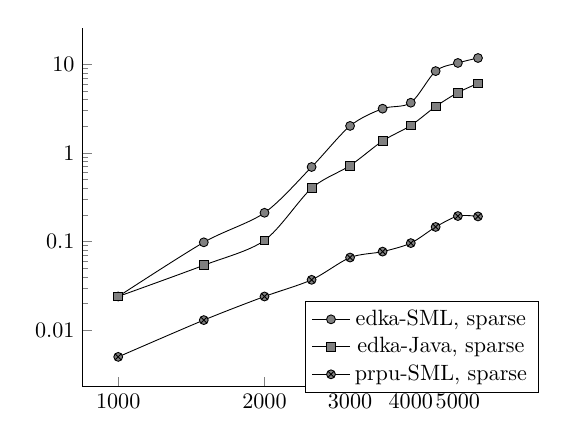
\begin{tikzpicture}[thick,scale=.8, every node/.style={scale=1}] %change the scales if you like to reduce the size
    \begin{axis}[
      %title={Benchmark of the Edmonds-Karp algorithm},
        axis x line*= bottom,
        axis y line*= left,
        xmode = log,
        ymode = log,
%         xlabel = Number of vertices in the network,
%         ylabel = Execution time in seconds, 
        xtick = {0,1000,...,5000},
        ytick = {0.01,0.1,1,10},
        xticklabels = {$1000$, $2000$, $3000$, $4000$, $5000$},
        yticklabels = {$0.01$,$0.1$,$1$,$10$}, 
        smooth,
        cycle list name = black white,
        legend style = { 
          at={(0.515,0.24)}, 
            anchor=north west,
            draw=black, 
            fill= white,
            align=left
        }
    ]
    
    %start data for plotting
      \addplot table {
        1000 .024   
        1500 .098  
        2000 .211  
        2500 .693  
        3000 2.014 
        3500 3.153 
        4000 3.679 
        4500 8.364 
        5000 10.328 
        5500 11.749    
      }; \addlegendentry{edka-SML, sparse};

      \addplot table {
        1000 .024   
        1500 .054   
        2000 .103  
        2500 .399  
        3000 .719  
        3500 1.362 
        4000 2.036 
        4500 3.334 
        5000 4.785 
        5500 6.079     
      }; \addlegendentry{edka-Java, sparse};

      \addplot table {
        1000 .005   
        1500 .013  
        2000 .024  
        2500 .037  
        3000 .066 
        3500 .077 
        4000 .096 
        4500 .146 
        5000 .194 
        5500 .192    
      }; \addlegendentry{prpu-SML, sparse};
    %end data for plotting
    \end{axis}
  \end{tikzpicture}
%
  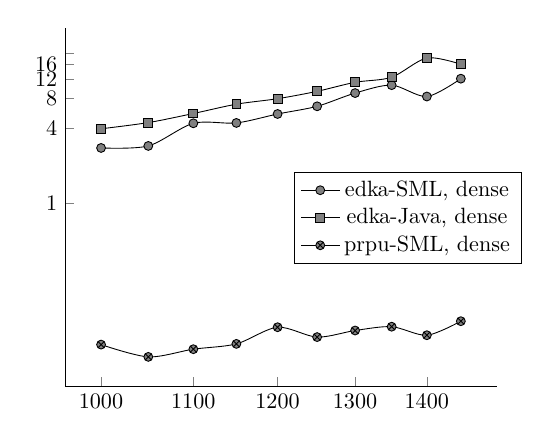
\begin{tikzpicture}[thick,scale=.8, every node/.style={scale=1}] %change the scales if you like to reduce the size
    \begin{axis}[
      %title={Benchmark of the Edmonds-Karp algorithm},
        axis x line*= bottom,
        axis y line*= left,
        xmode = log,
        ymode = log,
%         xlabel = Number of vertices in the network,
%         ylabel = Execution time in seconds, 
        xtick = {0,1000,1100,...,1400},
        ytick = {1,4,...,16},
        xticklabels = {$1000$, $1100$, $1200$, $1300$, $1400$}, 
        yticklabels = {$1$,$4$,$8$,$12$,$16$}, 
        smooth,
        cycle list name = black white,
        legend style = { 
          at={(0.53,0.6)}, 
            anchor=north west,
            draw=black, 
            fill= white,
            align=left
        }
    ]
    
    %start data for plotting
      \addplot table {
        1000	2.794
        1050	2.9
        1100	4.405
        1150	4.435
        1200	5.232
        1250	6.029
        1300	7.699
        1350	8.91
        1400	7.225
        1450	10.042 
      }; \addlegendentry{edka-SML, dense};

      \addplot table {
        1000	3.982
        1050	4.463
        1100	5.278
        1150	6.27
        1200	6.939
        1250	7.953
        1300	9.392
        1350	10.317
        1400	14.71
        1450	13.11  
      }; \addlegendentry{edka-Java, dense};

      \addplot table {
        1000	0.074
        1050	0.059
        1100	0.068
        1150	0.075
        1200	0.102
        1250	0.085
        1300	0.096
        1350	0.103
        1400	0.088
        1450	0.114  
      }; \addlegendentry{prpu-SML, dense};
    \end{axis}
  \end{tikzpicture}
%%%%%%%%%%%%%%%%%%%%%%%%%%%%%%%%%%%%%%%%%%%%%%%%%%%%%%%%%%%%%%%%%%
  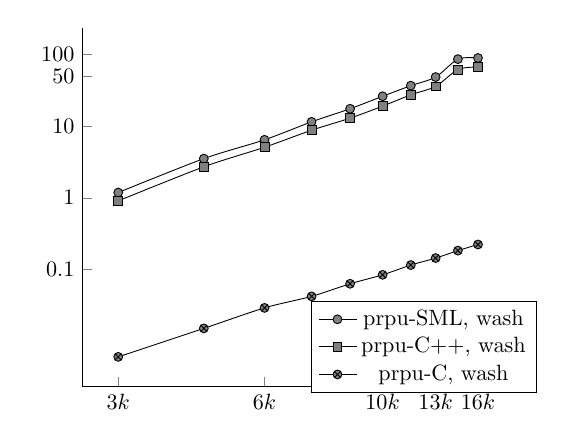
\begin{tikzpicture}[thick,scale=.8, every node/.style={scale=1}] %change the scales if you like to reduce the size
    \begin{axis}[
      %title={Benchmark of the Edmonds-Karp algorithm},
        axis x line*= bottom,
        axis y line*= left,
        xmode = log,
        ymode = log,
%         xlabel = Number of vertices in the network,
%         ylabel = Execution time in seconds, 
        xtick = {3000, 6000, 10500, 13500, 16500},
        ytick = {0.1,1,10,50,100},
        xticklabels = {$3k$, $6k$, $10k$, $13k$, $16k$},
        yticklabels = {$\text{\ \,}0.1$,$1$,$10$,$50$,$100$}, 
        smooth,
        cycle list name = black white,
        legend style = { 
          at={(0.53,0.24)}, 
            anchor=north west,
            draw=black, 
            fill= white,
            align=left
        }
    ]
    
    %start data for plotting


      \addplot table {
        3000	1.185
        4500	3.524
        6000	6.457
        7500	11.509
        9000	17.529
        10500	26.185
        12000	36.828
        13500	48.614
        15000	86.449
        16500	89.661
      }; \addlegendentry{prpu-SML, wash};

      \addplot table {
        3000	0.906
        4500	2.708
        6000	5.083
        7500	8.792
        9000	12.951
        10500	19.075
        12000	27.466
        13500	35.964
        15000	61.839
        16500	67.039
      }; \addlegendentry{prpu-C++, wash};

      \addplot table {
        3000	0.006
        4500	0.015
        6000	0.029
        7500	0.042
        9000	0.063
        10500	0.084
        12000	0.115
        13500	0.144
        15000	0.183
        16500	0.223
      }; \addlegendentry{prpu-C, wash};
    %end data for plotting
    \end{axis}
  \end{tikzpicture}
%%%%%%%%%%%%%%%%%%%%%%%%%%%%%%%%%%%%%%%%%%%%%%
  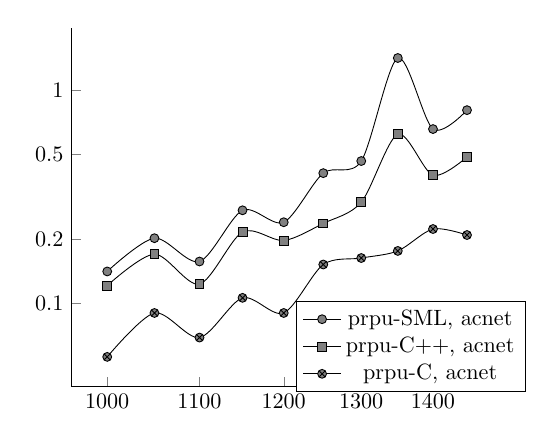
\begin{tikzpicture}[thick,scale=.8, every node/.style={scale=1}] %change the scales if you like to reduce the size
    \begin{axis}[
      %title={Benchmark of the Edmonds-Karp algorithm},
        axis x line*= bottom,
        axis y line*= left,
        xmode = log,
        ymode = log,
%         xlabel = Number of vertices in the network,
%         ylabel = Execution time in seconds, 
        xtick = {0,1000,1100,...,1400},
        ytick = {0.01, 0.1, 0.2, 0.5, 1},
        xticklabels = {$1000$, $1100$, $1200$, $1300$, $1400$}, 
        yticklabels = {$0.01$, $0.1$,$0.2$,$0.5$,$1$}, 
        smooth,
        cycle list name = black white,
        legend style = { 
          at={(0.52,0.24)}, 
            anchor=north west,
            draw=black, 
            fill= white,
            align=left
        }
    ]
    
    %start data for plotting
      \addplot table {
        1000	0.141
        1050	0.202
        1100	0.157
        1150	0.273
        1200	0.24
        1250	0.408
        1300	0.465
        1350	1.416
        1400	0.657
        1450	0.806
      }; \addlegendentry{prpu-SML, acnet};

      \addplot table {
        1000	0.121
        1050	0.17
        1100	0.123
        1150	0.216
        1200	0.197
        1250	0.237
        1300	0.298
        1350	0.621
        1400	0.399
        1450	0.486
      }; \addlegendentry{prpu-C++, acnet};

      \addplot table {
        1000	0.056
        1050	0.09
        1100	0.069
        1150	0.106
        1200	0.09
        1250	0.152
        1300	0.163
        1350	0.176
        1400	0.223
        1450	0.209
      }; \addlegendentry{prpu-C, acnet};
    \end{axis}
  \end{tikzpicture}
  %%%%%%%%%%%%%%%%%%%%%%%%%%%%%%%%%%%%%%%%%%%%%%
  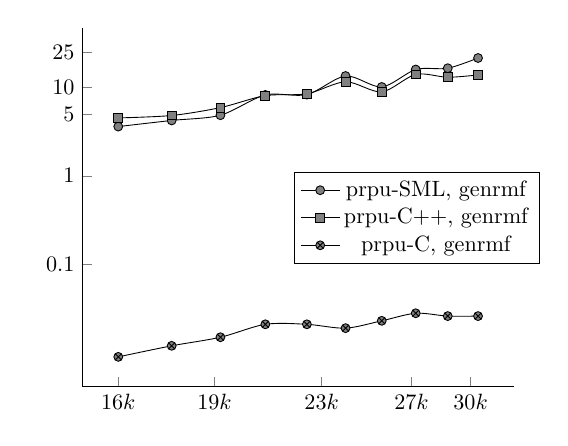
\begin{tikzpicture}[thick,scale=.8, every node/.style={scale=1}] %change the scales if you like to reduce the size
    \begin{axis}[
      %title={Benchmark of the Edmonds-Karp algorithm},
        axis x line*= bottom,
        axis y line*= left,
        xmode = log,
        ymode = log,
%         xlabel = Number of vertices in the network,
%         ylabel = Execution time in seconds, 
        xtick = {16000,19000,23000,27000,30000},
        ytick = {0.1,1,5,10,25},
        xticklabels = {$16k$, $19k$, $23k$, $27k$, $30k$}, 
        yticklabels = {$\text{\ \,}0.1$, $1$,$5$,$10$,$25$}, 
        smooth,
        cycle list name = black white,
        legend style = { 
          at={(0.49,0.6)}, 
            anchor=north west,
            draw=black, 
            fill= white,
            align=left
        }
    ]
    
    %start data for plotting
      \addplot table {
        16000	3.602
        17600	4.223
        19200	4.839
        20800	8.201
        22400	8.273
        24000	13.426
        25600	10.089
        27200	15.889
        28800	16.431
        30400	21.437
      }; \addlegendentry{prpu-SML, genrmf};

      \addplot table {
        16000	4.51
        17600	4.804
        19200	5.899
        20800	8.052
        22400	8.448
        24000	11.555
        25600	8.878
        27200	13.999
        28800	12.99
        30400	13.791
      }; \addlegendentry{prpu-C++, genrmf};

      \addplot table {
        16000	0.009
        17600	0.012
        19200	0.015
        20800	0.021
        22400	0.021
        24000	0.019
        25600	0.023
        27200	0.028
        28800	0.026
        30400	0.026
      }; \addlegendentry{prpu-C, genrmf};
    \end{axis}
  \end{tikzpicture}
  \caption{Benchmark of different implementations. The x-axis shows the number of nodes, the y axis the execution time in seconds.}\label{fig:benchmark}
  \end{figure}

  We observe that, for sparse graphs, the Java implementation is roughly faster by a factor of $1.6$, while for dense graphs, our implementation is faster by a factor of $1.2$. Note that the Java implementation operates on flows, while our implementation 
  operates on residual graphs (\cf Section~\ref{sec:impl_res_graph}). Moreover, the Java implementation does not store the augmenting 
  path in an intermediate list, but uses the predecessor map computed by the BFS directly (\cf Section~\ref{sec:impl_data_structures}).
  Finally note that a carefully optimized C++ implementation of the algorithm is only slightly faster than the Java implementation for sparse graphs,
  but roughly one order of magnitude faster for dense graphs. We leave it to future work to investigate this issue, and conclude that we were able to produce
  a reasonably fast verified implementation.
  
%   , without doing any low-level optimizations, but using the code as generated by the Isabelle/HOL code generator.
  
% 
%   What implementations did we compare: Authors? Where do implementations come from? 
%   [We must convince the reader that we did not intentionally chose bad implementations to compare us against!]
% 
%   Comparsion of algorithms (Modified data structure: Flow vs Flow-like vs ResGraph)
%     Computing successors in BFS: Filter by visited set first.
%       -> Technically more challenging, when computing on flow: 1 access first vs 2 accesses first. On resGraph: No advantage in memory accesses (However, plain array access vs. matrix access)
%     Computing bottleneck during BFS. Saves one iteration over the path, at the cost of one extra memory access per discovered node.
%     For our benchmarks, we observed that the BFS discovers considerably more nodes than the length of the ultimately returned path, 
%     and the overall code was faster with the extra iteration for bottleneck computation.
    
    

\section{Conclusion}\label{sec:concl}
  We have presented a verification of the Edmonds-Karp algorithm, using a stepwise refinement approach.
  Starting with a proof of the Ford-Fulkerson theorem, we have verified the generic Ford-Fulkerson method, 
  specialized it to the Edmonds-Karp algorithm, and proved the upper bound $O(VE)$ for the number of outer loop iterations.
  We then conducted several refinement steps to derive an efficiently executable implementation of the algorithm, 
  including a verified breadth first search algorithm to obtain shortest augmenting paths. 
  Finally, we added a verified algorithm to check whether the input is a valid network, and generated executable code in SML.
  The runtime of our verified implementation compares well to that of an unverified reference implementation in Java.
  
  Our formalization has combined several techniques to achieve an elegant and accessible formalization: 
  Using the Isar proof language~\cite{Wenzel99}, we were able to provide a completely rigorous but 
  still accessible proof of the Ford-Fulkerson theorem. The Isabelle Refinement Framework~\cite{LaTu12,La12} and the Sepref tool~\cite{La15,La16}
  allowed us to present the Ford-Fulkerson method on a level 
  of abstraction that closely resembles pseudocode presentations found in textbooks, and then formally link this presentation to an efficient
  implementation. Moreover, modularity of refinement allowed us to develop the breadth first search algorithm independently, and later link it to the 
  main algorithm. The BFS algorithm can be reused as building block for other algorithms. The data structures are re-usable, too: although we had to implement the array representation of (capacity) matrices for this project, it will be added to the growing library of verified imperative data structures 
  supported by the Sepref tool, such that it can be re-used for future formalizations.
  
  During this project, we have learned some lessons on verified algorithm development: 
  \begin{itemize}
  \item It is important to keep the levels of abstraction strictly separated.
    For example, when implementing the capacity function with arrays, one needs to show that it is only applied to valid nodes.
    However, proving that, e.g., augmenting paths only contain valid nodes is hard at this low level. 
    Instead, one can protect the application of the capacity function by an assertion --- already on a high abstraction level where it can be easily discharged. 
    On refinement, this assertion is passed down, and ultimately available for the implementation.
    Optimally, one wraps the function together with an assertion of its precondition into a new constant, which is then refined independently.
  \item Profiling has helped a lot in identifying candidates for optimization. For example, based on profiling data, we decided to delay a 
    possible deforestation optimization on augmenting paths, and to first refine the algorithm to operate on residual graphs directly.
  \item ``Efficiency bugs'' are as easy to introduce as for unverified software. For example, out of convenience, we implemented the successor list computation by
    \emph{filter}. Profiling then indicated a hot-spot on this function. As the order of successors does not matter, we invested a bit more work to make the computation tail 
    recursive and gained a significant speed-up. Moreover, we realized only lately that we had accidentally implemented and verified
    matrices with column major ordering, which have a poor cache locality for our algorithm. Changing the order resulted in another significant speed-up.
  \end{itemize}
  
  We conclude with some statistics:
  The formalization consists of roughly 13000 lines of proof text, where the graph theory up to the Ford-Fulkerson algorithm requires 3000 lines.
  The abstract Edmonds-Karp algorithm and its complexity analysis contribute 800 lines, and its implementation (including BFS) another 1700 lines.
  The generic push relabel algorithm and its complexity analysis is 1700 lines, the abstract implementations of relabel-to-front and FIFO push-relabel is another 1000 lines,
  and their refinement to an efficient implementation takes 2000 lines.
  
  The remaining lines are contributed by the network checker and some auxiliary theories. The development of the theories required roughly 5 man month, a significant amount of this time going into a first, purely functional implementation of the Edmonds-Karp algorithm, which was later dropped in favor of the faster imperative version.
  
  
  \subsection{Related Work}\label{sec:related_work}
  We are only aware of one other formalization of the Ford-Fulkerson method conducted in Mizar~\cite{MaRu05} by Lee. Unfortunately, there seems to be no publication
  on this formalization except~\cite{Lee05}, which provides a Mizar proof script without any additional comments except that it ``defines and proves correctness of Ford/Fulkerson's Maximum Network-Flow algorithm at the level of graph manipulations''. Moreover, in Lee et al.~\cite{LeRu07}, which is about graph representation in Mizar, the formalization is shortly mentioned, and it is clarified that it does not provide any implementation or data structure formalization.
  As far as we understood the Mizar proof script, it formalizes an algorithm roughly equivalent to our abstract version of the Ford-Fulkerson method.
  Termination is only proved for integer valued capacities.
  
  Apart from our own work~\cite{La14,NoLa12}, there are several other verifications of graph algorithms and their implementations, using different techniques and proof assistants. Noschinski~\cite{Nosch15} verifies a checker for (non-)planarity certificates using a bottom-up approach. Starting at a C implementation,
  the AutoCorres tool~\cite{Greenaway15,GAK12} generates a monadic representation of the program in Isabelle. Further abstractions are applied
  to hide low-level details like pointer manipulations and fixed size integers. Finally, a verification condition
  generator is used to prove the abstracted program correct. Note that their approach takes the opposite direction than ours: While they start at a concrete version of the algorithm and use abstraction steps to eliminate implementation details, we start at an abstract version, and use concretization steps to introduce implementation details.

  Chargu\'eraud~\cite{char11} also uses a bottom-up approach to verify imperative programs written in a subset of OCaml, amongst them a version of Dijkstra's algorithm:
  A verification condition generator generates a \emph{characteristic formula}, which reflects the semantics of the program in the logic of the Coq proof assistant~\cite{BeCa10}.
  
  \subsection{Future Work}
  While we implemented a simple version of the push-relabel algorithm, there are more advanced implementations, like the one of Cherkassky et el.~\cite{ChGo97} that 
  we also use in the benchmarks. The same authors also provide an implementation based on the highest label selection rule, which is reported to be even more efficient 
  in practice. Our formalized algorithm misses two important heuristics of these advanced algorithms: First, the global relabeling heuristics periodically performs a breadth first search on the reversed residual graph, to determine exact node labels based on their distance to the sink. Second, the algorithm is split in two phases: 
  The first phase ignores nodes with labels greater $|V|$, and already determines the exact value of the flow. The second phase only pushes excess flow back to the source. 
  Using different heuristics for both phases is reported to improve practical performance~\cite{ChGo97}. 
  Thus, the main focus of future work will be to verify these heuristics in order to obtain more efficient verified algorithms.
  


%\section{Introduction}
%\label{intro}
%Your text comes here. Separate text sections with
%\section{Section title}
%\label{sec:1}
%\subsection{Subsection title}
%\label{sec:2}
%as required. Don't forget to give each section
%and subsection a unique label (see Sect.~\ref{sec:1}).
%\paragraph{Paragraph headings} Use paragraph headings as needed.
%\begin{equation}
%a^2+b^2=c^2
%\end{equation}
%
%% For one-column wide figures use
%\begin{figure}
%% Use the relevant command to insert your figure file.
%% For example, with the graphicx package use
%  %\includegraphics{example.eps}
%% figure caption is below the figure
%\caption{Please write your figure caption here}
%\label{fig:1}       % Give a unique label
%\end{figure}
%%
%% For two-column wide figures use
%\begin{figure*}
%% Use the relevant command to insert your figure file.
%% For example, with the graphicx package use
% % \includegraphics[width=0.75\textwidth]{example.eps}
%% figure caption is below the figure
%\caption{Please write your figure caption here}
%\label{fig:2}       % Give a unique label
%\end{figure*}
%%
%% For tables use
%\begin{table}
%% table caption is above the table
%\caption{Please write your table caption here}
%\label{tab:1}       % Give a unique label
%% For LaTeX tables use
%\begin{tabular}{lll}
%\hline\noalign{\smallskip}
%first & second & third  \\
%\noalign{\smallskip}\hline\noalign{\smallskip}
%number & number & number \\
%number & number & number \\
%\noalign{\smallskip}\hline
%\end{tabular}
%\end{table}
%
%
%%\begin{acknowledgements}
%%If you'd like to thank anyone, place your comments here
%%and remove the percent signs.
%%\end{acknowledgements}
%
%% BibTeX users please use one of
%%\bibliographystyle{spbasic}      % basic style, author-year citations
%%\bibliographystyle{spmpsci}      % mathematics and physical sciences
%%\bibliographystyle{spphys}       % APS-like style for physics
%%\bibliography{}   % name your BibTeX data base
%
%% Non-BibTeX users please use
%%\begin{thebibliography}{}
%%
%% and use \bibitem to create references. Consult the Instructions
%% for authors for reference list style.
%%
%%\bibitem{RefJ}
%% Format for Journal Reference
%%Author, Article title, Journal, Volume, page numbers (year)
%% Format for books
%%\bibitem{RefB}
%%Author, Book title, page numbers. Publisher, place (year)
%% etc
%% \end{thebibliography}

\bibliographystyle{abbrv}
\bibliography{root}

\end{document}

